\documentclass[12pt,a4paper]{report}

% ---------- Paket dasar ----------
\usepackage[utf8]{inputenc}
\usepackage[T1]{fontenc}
\usepackage[indonesian]{babel}
\usepackage{lipsum}

% ---------- Paket matematika & gambar ----------
\usepackage{amsmath,amssymb}
\usepackage{graphicx}
\usepackage{caption}
\usepackage{subcaption}
\usepackage{float}
\bibliographystyle{IEEEtran}
% ---------- Paket lain ----------
\usepackage[most]{tcolorbox}
\usepackage{forest}
\usepackage{hyperref}
\usepackage{fancyhdr}

\usepackage{titlesec}

\usepackage{titlesec}
\usepackage{longtable}
\usepackage{array} % untuk menentukan lebar kolom
\usepackage{booktabs} % gaya tabel lebih elegan
\usepackage[table]{xcolor}



% Tambah jarak aman dari header dan footer:	
\setlength{\headheight}{10pt}   % wajib cukup besar untuk fancyhdr
\setlength{\headsep}{55pt}      % jarak header ke teks
\setlength{\footskip}{28pt}     % jarak teks ke footer
\usepackage[a4paper,top=3cm,bottom=3cm,left=3cm,right=3cm]{geometry}

% Semua gambar dari folder public dan subfoldernya
\graphicspath{{public/}{public/01-pendahuluan/}{public/02-dasar-teori/}{public/03-implementasi/}}

% --- Pengaturan header & footer ---
\pagestyle{fancy}
\fancyhf{} % clear all

% --- Paksa semua halaman (termasuk awal chapter) memakai fancy ---
\fancypagestyle{plain}{%
	\fancyhf{}%
	\fancyhead[L]{%
		
\includegraphics[height=1.1cm]{logo-itb}\hspace{0.3cm}%
		
\includegraphics[height=1.1cm]{logo-stei}\hspace{0.3cm}%
	}%
	\fancyhead[R]{%
		\begin{minipage}{9cm}
			\raggedleft\bfseries IF 2211 Strategi Algoritma\\
			\normalsize Laporan Akhir Tugas Besar 3\\
			Semester Genap 2025/2026
		\end{minipage}
	}%
	\renewcommand{\headrulewidth}{0.4pt}%
	\fancyfoot[L]{\small v1.0}%
	\fancyfoot[C]{\small Halaman \thepage}%
	\fancyfoot[R]{\small }%
	\renewcommand{\footrulewidth}{0.4pt}%
}


\fancyhead[L]{%
	
\includegraphics[height=1.5cm]{logo-itb}\hspace{0.3cm}%
	
\includegraphics[height=1.5cm]{logo-stei}\hspace{0.3cm}%
}

\fancyhead[R]{%
	\begin{minipage}{9cm}
		\raggedleft\bfseries IF2211 Strategi Algoritma\\
		\normalsize Laporan Akhir Tugas Besar 3\\
		\itshape Semester Genap 2025/2026
	\end{minipage}
}

\renewcommand{\headrulewidth}{0.4pt}

\fancyfoot[L]{\small v1.0}
\fancyfoot[C]{\small Halaman \thepage}
\fancyfoot[R]{\small }
\renewcommand{\footrulewidth}{0.4pt}

\begin{document}
	
	\begin{titlepage}
		\thispagestyle{empty}
		\centering
		
		% ---------- Judul utama ----------
		{\LARGE \textbf{Tugas Besar 2}\par}
		\vspace{0.2cm}
		{\LARGE \textbf{Pasti-Gacor-Zeus}\par}
		\vspace{0.8cm}
		{\large IF2211 Strategi Algoritma\par}
		\vspace{0.2cm}
		{\large Implementasi Pattern Matching pada Chromium Browser Extension untuk Deteksi Judi
Online\par}
		\vspace{0.2cm}
		{\large Semester 2 Tahun 2025/2026\par}
		
		% ---------- Gambar tengah ----------
		\vspace{1.8cm}
		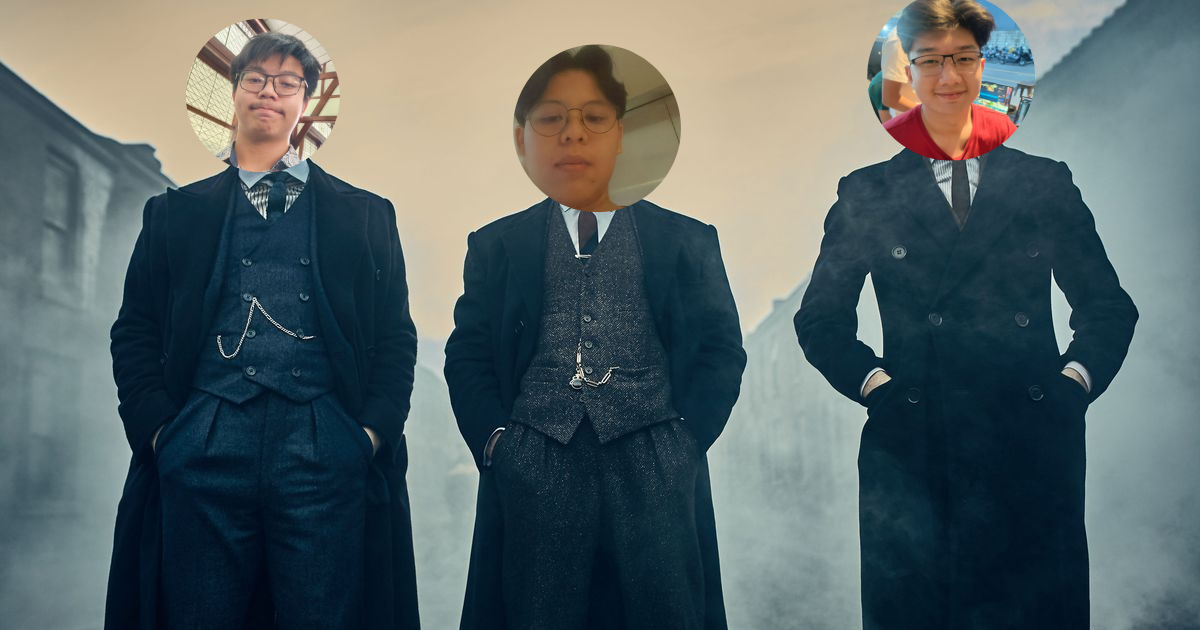
\includegraphics[width=0.9\textwidth]{foto-kelompok}\par
		
		% ---------- Disusun oleh ----------
		\vspace{1.2cm}
		{\bfseries Disusun oleh:\par}
		\vspace{0.2cm}
		\textbf{Pasti-Gacor-Zeus}
		\vspace{0.5cm} \\
		\begin{tabular}{l l}
			Athilla Zaidan Zidna Fann & (13524068) \\
			Stevanus Agustav Wongso & (13524020) \\
			Ray Owen Martin & (13524033) \\
		\end{tabular}
		
		% ---------- Institusi ----------
		\vspace{2.0cm}
		Laboratorium Ilmu dan Rekayasa Komputasi\par
		Program Studi Teknik Informatika\par
		Sekolah Teknik Elektro dan Informatika\par
		Institut Teknologi Bandung\par
		
	\end{titlepage}
	
	\clearpage
	\pagestyle{fancy}
	
	\tableofcontents
	\clearpage
	
	\chapter{Pendahuluan}
	\section{Kisah}

Perkembangan web membuat informasi dapat disebarkan dengan sangat cepat.
Halaman web, media sosial, forum, dan situs promosi dapat memuat berbagai
jenis konten hanya dalam hitungan detik. Di sisi lain, kemudahan penyebaran
informasi juga membuka ruang bagi munculnya konten berisiko, salah satunya
konten yang berkaitan dengan judi daring atau \textit{judi online} (judol).
Konten seperti ini sering kali muncul dalam bentuk kata kunci eksplisit,
variasi penulisan, angka yang disisipkan ke dalam kata, hingga teks yang
tertanam di dalam gambar.

Deteksi manual terhadap konten judol tidak selalu praktis. Sebuah halaman web
dapat memiliki banyak elemen teks, tautan, gambar promosi, dan istilah yang
sengaja dimodifikasi agar tidak mudah ditemukan oleh pencarian biasa. Sebagai
contoh, kata seperti \texttt{gacor} dapat ditulis menjadi \texttt{g4cor},
\texttt{slot} dapat muncul sebagai bagian dari frasa promosi, dan nama situs
dapat ditulis dengan pola huruf diikuti angka seperti \texttt{ZEUS222}.
Variasi semacam ini membuat pencocokan kata secara eksak saja tidak cukup.

Permasalahan tersebut dapat dipandang sebagai persoalan pencocokan string.
Sebuah sistem perlu membaca teks pada halaman web, membandingkannya dengan
daftar kata kunci yang dicurigai, mengenali pola tertentu menggunakan
\textit{regular expression}, serta mendeteksi bentuk penulisan yang mirip
melalui pendekatan \textit{approximate string matching}. Selain itu, karena
sebagian konten promosi muncul dalam gambar, sistem juga perlu memiliki
kemampuan \textit{Optical Character Recognition} (OCR) agar teks pada gambar
dapat diproses oleh pipeline deteksi yang sama.

Pada Tugas Besar ini, dikembangkan sebuah ekstensi Chromium bernama
\textbf{Judol Detector}. Ekstensi ini melakukan pemindaian terhadap teks yang
terlihat pada halaman web, mendeteksi indikasi konten judol menggunakan
kombinasi algoritma pencocokan string, menandai teks yang terdeteksi secara
langsung pada halaman, serta menampilkan statistik hasil deteksi melalui popup
ekstensi. Program juga menyediakan mode blur untuk menyamarkan konten yang
terdeteksi dan fitur OCR untuk memindai teks yang tertanam pada gambar.

\section{Latar Belakang}

Pencocokan string merupakan salah satu persoalan mendasar dalam ilmu komputer.
Dalam bentuk paling sederhana, pencocokan string bertujuan menemukan kemunculan
suatu pola dalam teks. Persoalan ini banyak digunakan dalam mesin pencari,
editor teks, bioinformatika, keamanan siber, dan sistem moderasi konten.
Algoritma klasik seperti Knuth-Morris-Pratt (KMP) dan Boyer-Moore dirancang
untuk melakukan pencocokan eksak secara efisien dengan mengurangi jumlah
perbandingan karakter yang tidak perlu \cite{cormen2009introduction}.

Pada konteks deteksi konten judol, pencocokan eksak berguna untuk menemukan
kata atau frasa yang sudah diketahui, seperti \texttt{slot}, \texttt{rtp},
\texttt{bonus deposit}, atau \texttt{situs judi}. Namun, konten promosi sering
menggunakan variasi penulisan untuk menghindari deteksi sederhana. Penulisan
seperti \texttt{H0KI88}, \texttt{G4COR}, atau \texttt{SLOT777} tetap dapat
dimaknai oleh manusia sebagai istilah judol, meskipun tidak sama persis dengan
kata kunci dasar. Oleh karena itu, diperlukan pendekatan lain seperti
\textit{regular expression} dan \textit{fuzzy matching}.

\textit{Regular expression} dapat digunakan untuk mendeteksi pola tekstual
yang terstruktur, misalnya gabungan huruf dan angka yang sering digunakan pada
nama situs atau kode promosi \cite{friedl2006regex}. Sementara itu,
\textit{Levenshtein Distance} mengukur jarak edit antara dua string berdasarkan
jumlah operasi penyisipan, penghapusan, dan penggantian karakter yang
diperlukan untuk mengubah satu string menjadi string lain \cite{levenshtein1966}.
Dengan memberikan bobot khusus pada karakter yang mirip secara visual, sistem
dapat mengenali variasi seperti huruf \texttt{o} yang diganti angka
\texttt{0}, huruf \texttt{a} yang diganti angka \texttt{4}, atau huruf
\texttt{s} yang diganti angka \texttt{5}.

Web modern juga tidak hanya memuat teks dalam bentuk node DOM. Banyak konten
promosi disisipkan dalam gambar, banner, atau elemen visual. Untuk menangani
kasus tersebut, Judol Detector menggunakan OCR berbasis Tesseract.js untuk
mengambil teks dari gambar yang terlihat pada halaman \cite{tesseractjs}.
Teks hasil OCR kemudian diproses menggunakan pipeline deteksi yang sama dengan
teks DOM.

Pemilihan bentuk ekstensi browser memungkinkan deteksi dilakukan langsung pada
halaman yang sedang dibuka pengguna. Dengan Manifest V3, ekstensi Chromium
dapat menjalankan \textit{content script} untuk berinteraksi dengan halaman,
serta menyediakan popup sebagai antarmuka ringkas untuk menampilkan status dan
statistik pemindaian \cite{chrome_extensions}. Pendekatan ini membuat sistem
tidak perlu mengunduh halaman melalui server terpisah, melainkan bekerja di
sisi klien pada halaman yang sedang aktif.

\section{Deskripsi Tugas}

Program Judol Detector adalah ekstensi Chromium untuk mendeteksi indikasi
konten judi daring pada halaman web. Program memindai teks yang terlihat pada
halaman, menjalankan algoritma pencocokan terhadap daftar kata kunci, menandai
hasil deteksi pada halaman, dan menampilkan ringkasan statistik melalui popup.

Secara umum, alur kerja program adalah sebagai berikut:

\begin{enumerate}
    \item Pengguna membuka halaman web yang ingin diperiksa.
    \item Pengguna membuka popup ekstensi dan menjalankan proses pemindaian.
    \item \textit{Content script} mengumpulkan node teks yang terlihat pada DOM.
    \item Program menjalankan pipeline deteksi, yaitu pencocokan pola dengan
    RegEx dan pencocokan fuzzy dengan Weighted Levenshtein.
    \item Jika OCR diaktifkan, program juga memindai gambar yang terlihat,
    melakukan preprocessing citra, dan menjalankan pipeline deteksi terhadap
    teks hasil OCR.
    \item Teks atau gambar yang terdeteksi diberi penanda visual pada halaman.
    \item Popup menampilkan jumlah hasil deteksi, waktu eksekusi, perbandingan
    algoritma, kata kunci paling sering muncul, dan ringkasan OCR.
\end{enumerate}

Program dikembangkan menggunakan TypeScript, React, Vite, Tailwind CSS, dan
Tesseract.js. TypeScript digunakan untuk menjaga struktur data deteksi,
React digunakan untuk membangun antarmuka popup, Vite digunakan sebagai build
tool, Tailwind CSS digunakan untuk styling, dan Tesseract.js digunakan untuk
fitur OCR.

\subsection{Masukan}

Masukan yang digunakan oleh program terdiri atas beberapa komponen berikut:

\begin{enumerate}
    \item \textbf{Halaman web aktif}, yaitu halaman yang sedang dibuka pada
    browser Chromium dan menjadi target pemindaian.

    \item \textbf{Teks DOM yang terlihat}, yaitu kumpulan node teks yang dapat
    dibaca dari struktur DOM halaman dan tidak berada pada elemen yang harus
    diabaikan seperti \texttt{script}, \texttt{style}, \texttt{textarea}, dan
    \texttt{input}.

    \item \textbf{Daftar kata kunci}, yaitu kumpulan istilah yang berkaitan
    dengan judol, seperti \texttt{slot}, \texttt{gacor}, \texttt{rtp},
    \texttt{jackpot}, \texttt{casino online}, dan berbagai variasi frasa
    promosi lain.

    \item \textbf{Gambar halaman}, yaitu elemen gambar yang terlihat pada
    viewport dan dapat diproses melalui OCR setelah melalui tahap preprocessing.

    \item \textbf{Pengaturan popup}, yaitu pilihan pengguna seperti menjalankan
    ulang pemindaian, mengaktifkan OCR, dan mengaktifkan blur terhadap konten
    yang terdeteksi.
\end{enumerate}

\subsection{Keluaran}

Keluaran yang dihasilkan program adalah sebagai berikut:

\begin{enumerate}
    \item \textbf{Highlight pada halaman}, yaitu penandaan visual pada teks
    yang terdeteksi sebagai indikasi konten judol.

    \item \textbf{Blur konten}, yaitu penyamaran visual terhadap teks atau
    gambar yang terdeteksi ketika fitur blur diaktifkan atau ketika gambar
    hasil OCR dinyatakan positif.

    \item \textbf{Tooltip deteksi}, yaitu informasi tambahan yang muncul saat
    pengguna mengarahkan kursor ke hasil deteksi, berisi kata kunci,
    algoritma, jumlah kemunculan, dan waktu eksekusi.

    \item \textbf{Ringkasan statistik}, yaitu jumlah total deteksi, waktu
    eksekusi, jumlah deteksi per algoritma, dan daftar kata kunci yang paling
    sering ditemukan.

    \item \textbf{Ringkasan OCR}, yaitu jumlah gambar yang dipindai, jumlah
    gambar yang terdeteksi positif, jumlah gambar yang dilewati, dan waktu
    eksekusi OCR.

    \item \textbf{Status pemindaian}, yaitu status seperti siap, sedang
    memindai, terdeteksi, bersih, atau gagal memindai.
\end{enumerate}

	
	\chapter{Dasar Teori}
	Bagian ini menjelaskan teori yang menjadi dasar pengembangan Judol Detector.
Konsep yang dibahas meliputi ekstensi browser, DOM, pencocokan string,
\textit{regular expression}, Weighted Levenshtein Distance, OCR, serta
mekanisme penandaan hasil deteksi pada halaman web.

\section{Ekstensi Browser Chromium}

Ekstensi browser adalah perangkat lunak tambahan yang berjalan di dalam
peramban untuk menambah atau memodifikasi perilaku halaman web. Pada Chromium,
ekstensi didefinisikan melalui file \texttt{manifest.json} yang memuat
metadata, permission, script, dan konfigurasi antarmuka \cite{chrome_extensions}.

Manifest V3 memisahkan beberapa komponen utama:

\begin{itemize}
    \item \textbf{Popup}, yaitu antarmuka kecil yang muncul ketika pengguna
    menekan ikon ekstensi.
    \item \textbf{Content script}, yaitu script yang disisipkan ke halaman web
    dan dapat membaca atau memodifikasi DOM halaman.
    \item \textbf{Permission}, yaitu izin yang diperlukan ekstensi, misalnya
    izin membaca tab aktif, menyimpan data lokal, atau mengeksekusi script.
\end{itemize}

Pada Judol Detector, popup digunakan untuk menampilkan statistik dan kontrol
pemindaian, sedangkan content script digunakan untuk mengambil teks halaman,
menjalankan highlight, dan memberi efek blur pada konten yang terdeteksi.

\section{Document Object Model}

\textit{Document Object Model} (DOM) adalah representasi struktur dokumen HTML
dalam bentuk pohon hierarkis \cite{mdn_dom}. Setiap elemen HTML, teks, dan
atribut dapat direpresentasikan sebagai node. Melalui DOM, script dapat membaca
isi halaman, mencari elemen tertentu, dan memodifikasi tampilan halaman secara
dinamis.

Dalam Judol Detector, DOM digunakan untuk dua keperluan utama. Pertama, content
script menelusuri DOM untuk menemukan node teks yang terlihat dan relevan untuk
dipindai. Kedua, setelah sebuah teks terdeteksi, node teks tersebut diganti
dengan elemen \texttt{span} khusus agar hasil deteksi dapat diberi highlight,
tooltip, dan blur.

Tidak semua node teks perlu dipindai. Teks yang berada pada elemen seperti
\texttt{script}, \texttt{style}, \texttt{noscript}, \texttt{textarea}, dan
\texttt{input} diabaikan karena tidak merepresentasikan konten halaman yang
umumnya dibaca pengguna. Pemfilteran ini membuat proses pemindaian lebih fokus
pada teks yang benar-benar tampil pada halaman.

\section{Pencocokan String}

Pencocokan string adalah proses mencari kemunculan suatu pola dalam teks.
Jika diberikan teks $T$ dengan panjang $n$ dan pola $P$ dengan panjang $m$,
tujuan pencocokan string adalah menemukan indeks pada $T$ di mana $P$ muncul.
Persoalan ini merupakan dasar dari banyak aplikasi pemrosesan teks, termasuk
deteksi kata kunci \cite{cormen2009introduction}.

Dalam konteks deteksi judol, pola yang dicari adalah daftar kata kunci seperti
\texttt{slot}, \texttt{gacor}, \texttt{rtp}, \texttt{jackpot}, dan frasa lain
yang berkaitan dengan promosi judi daring. Pencocokan dapat dilakukan secara
eksak maupun tidak eksak. Pencocokan eksak hanya menerima string yang sama
persis, sedangkan pencocokan tidak eksak menerima string yang mirip berdasarkan
ukuran tertentu.

\section{Regular Expression}

\textit{Regular expression} (RegEx) adalah notasi untuk mendeskripsikan pola
teks. RegEx memungkinkan pencarian tidak hanya berdasarkan kata tetap, tetapi
juga berdasarkan struktur karakter tertentu \cite{friedl2006regex}. Contohnya,
pola huruf yang diikuti angka dapat digunakan untuk mendeteksi nama situs atau
kode promosi yang ditulis seperti \texttt{SLOT88}, \texttt{ZEUS222}, atau
\texttt{MAXWIN234}.

Pada Judol Detector, RegEx digunakan untuk mendeteksi pola kata yang terdiri
atas minimal dua huruf dan diikuti dua hingga tiga angka. Pola ini menangkap
format umum yang sering muncul pada konten promosi judol, terutama ketika nama
brand atau istilah promosi digabungkan dengan angka.

Secara konseptual, pola yang digunakan dapat dijelaskan sebagai berikut:

\begin{table}[H]
\centering
\caption{Komponen pola RegEx}
\label{tab:regex-pattern}
\begin{tabular}{|p{4cm}|p{9cm}|}
\hline
\textbf{Komponen} & \textbf{Makna} \\
\hline
Batas kiri token & Memastikan pola tidak berada di tengah kata lain. \\
\hline
Huruf minimal dua karakter & Menangkap bagian nama atau istilah promosi. \\
\hline
Angka dua sampai tiga digit & Menangkap akhiran numerik seperti \texttt{88}, \texttt{777}, atau \texttt{222}. \\
\hline
Batas kanan token & Memastikan pola berakhir sebagai token utuh. \\
\hline
\end{tabular}
\end{table}

\section{Levenshtein Distance}

\textit{Levenshtein Distance} adalah ukuran jarak antara dua string berdasarkan
jumlah minimum operasi edit yang diperlukan untuk mengubah satu string menjadi
string lain \cite{levenshtein1966}. Operasi edit yang umum digunakan adalah:

\begin{enumerate}
    \item penyisipan karakter,
    \item penghapusan karakter,
    \item penggantian karakter.
\end{enumerate}

Jika jarak edit antara dua string kecil, maka kedua string dianggap mirip.
Sebagai contoh, kata \texttt{gacor} dan \texttt{g4cor} hanya berbeda pada satu
karakter jika angka \texttt{4} dianggap sebagai pengganti huruf \texttt{a}.

\subsection{Weighted Levenshtein Distance}

Weighted Levenshtein Distance adalah variasi Levenshtein Distance yang memberi
bobot berbeda pada operasi edit tertentu. Pada Judol Detector, penggantian
karakter yang mirip secara visual diberi biaya lebih kecil dibandingkan
penggantian karakter biasa. Pendekatan ini digunakan karena banyak konten judol
memodifikasi kata dengan karakter yang tampak mirip.

\begin{table}[H]
\centering
\caption{Contoh karakter yang dianggap mirip secara visual}
\label{tab:visual-substitution}
\begin{tabular}{|p{4cm}|p{8cm}|}
\hline
\textbf{Huruf} & \textbf{Variasi visual} \\
\hline
\texttt{o} & \texttt{0} \\
\hline
\texttt{a} & \texttt{4} \\
\hline
\texttt{i} & \texttt{1}, \texttt{l}, \texttt{|} \\
\hline
\texttt{e} & \texttt{3} \\
\hline
\texttt{s} & \texttt{5}, \texttt{\$} \\
\hline
\texttt{b} & \texttt{8} \\
\hline
\texttt{g} & \texttt{6}, \texttt{9} \\
\hline
\texttt{t} & \texttt{7} \\
\hline
\end{tabular}
\end{table}

Nilai kemiripan dihitung dari jarak edit berbobot. Jika nilai kemiripan
melebihi ambang batas tertentu, token pada halaman dianggap cocok dengan kata
kunci. Pada implementasi program, ambang batas default yang digunakan adalah
0,78. Nilai ini dipilih agar sistem cukup sensitif terhadap variasi penulisan,
tetapi tetap membatasi jumlah hasil positif palsu.

\section{Boyer-Moore}

Algoritma Boyer-Moore adalah salah satu algoritma pencocokan string yang
bekerja dengan membandingkan karakter dari kanan ke kiri. Inti dari algoritma
ini adalah menggunakan \textit{bad character heuristic} untuk menentukan seberapa
jauh pola digeser ketika terjadi ketidakcocokan.

\begin{quotation}
Inti dari \textit{bad character heuristic} cukup simpel. Ketika kita
membandingkan pola dengan teks dan menemukan karakter yang tidak cocok, karakter
di teks tersebut disebut \textit{bad character} . Begitu
terjadi ketidakcocokan, pola tidak digeser sedikit demi sedikit, melainkan
langsung ``dilompatkan'' sejauh mungkin. Ada dua kemungkinan pergeseran:
pertama, pola digeser hingga karakter buruk di teks bisa cocok dengan
kemunculan terakhirnya di dalam pola; kedua, jika karakter tersebut sama
sekali tidak ada di pola, maka pola langsung dilewati melewati karakter yang
tidak cocok itu.
\cite{geeksforgeeks_boyer_moore}
\end{quotation}

Dengan heuristic ini, algoritma dapat melompati sejumlah posisi yang tidak
perlu diperiksa, sehingga pada kasus terbaik kompleksitasnya mendekati $O(n/m)$.


\subsection{Algoritma Rabin-Karp}

Berbeda dengan algoritma pencocokan string yang membandingkan karakter satu per
satu secara langsung, algoritma Rabin-Karp menggunakan fungsi hash untuk
mempercepat pencarian. Ide utamanya adalah menghitung nilai hash dari pola, lalu
membandingkannya dengan hash setiap jendela teks yang berukuran sama dengan
pola. Jika hash cocok, barulah dilakukan pemeriksaan karakter demi karakter
untuk memastikan tidak terjadi \textit{hash collision}
\cite{geeksforgeeks_rabin_karp}.

Untuk menghitung hash, setiap karakter dianggap sebagai digit dalam sistem
bilangan berbasis $d$ (biasanya 256 untuk ASCII), lalu nilai tersebut diambil
modulo sebuah bilangan prima $q$. Modulo ini berfungsi untuk mencegah
\textit{overflow} dan mengurangi kemungkinan tabrakan hash. Agar tidak perlu
menghitung ulang dari nol setiap kali jendela bergeser, algoritma ini
menggunakan teknik \textit{rolling hash}: karakter paling kiri dikeluarkan,
sisa nilai dikalikan ulang dengan basis, lalu karakter baru di kanan
dimasukkan. Dengan cara ini, hash jendela berikutnya bisa diperoleh dalam waktu
konstan.

Pada kasus rata-rata, algoritma ini berjalan dengan kompleksitas $O(n + m)$
karena setiap pergeseran hanya melakukan satu kali operasi aritmetika. Namun,
pada kasus terburuk ketika banyak tabrakan hash terjadi, kompleksitasnya bisa
naik menjadi $O(n \times m)$ karena setiap tabrakan harus diverifikasi secara
manual karakter per karakter.

\section{Tokenisasi Teks}

Sebelum pencocokan fuzzy dilakukan, teks perlu dipecah menjadi kandidat token.
Token adalah potongan teks yang berisi huruf, angka, garis bawah, atau beberapa
simbol yang relevan. Tokenisasi memungkinkan program membandingkan kata kunci
dengan bagian teks yang berukuran sebanding.

Untuk kata kunci yang terdiri atas beberapa kata, seperti \texttt{slot gacor}
atau \texttt{bonus deposit}, program membentuk jendela token dengan jumlah
token yang sama dengan jumlah token pada kata kunci. Dengan cara ini, frasa
multi-kata tetap dapat dibandingkan menggunakan Weighted Levenshtein.

\section{Deduplication dan Cache}

Pipeline deteksi dapat menghasilkan lebih dari satu hasil pada rentang teks
yang sama, misalnya ketika satu token cocok oleh RegEx dan juga cocok oleh
Weighted Levenshtein. Oleh karena itu, program melakukan deduplikasi berdasarkan
rentang indeks awal dan akhir dari hasil deteksi. Hasil yang memiliki rentang
sama hanya disimpan sekali.

Program juga menggunakan cache untuk menyimpan hasil pemindaian teks. Cache
menghindari penghitungan ulang terhadap teks, daftar kata kunci, dan opsi
deteksi yang sama. Dengan demikian, pemindaian berulang pada halaman yang sama
dapat dilakukan lebih efisien.

\section{Optical Character Recognition}

\textit{Optical Character Recognition} (OCR) adalah proses mengenali teks dari
gambar. OCR berguna ketika teks tidak tersedia sebagai node DOM, melainkan
menjadi bagian dari banner, poster, atau gambar promosi. Pada Judol Detector,
OCR dilakukan menggunakan Tesseract.js, yaitu port JavaScript dari mesin OCR
Tesseract \cite{tesseractjs}.

Proses OCR pada program terdiri atas beberapa tahap:

\begin{enumerate}
    \item memilih gambar atau elemen visual yang terlihat pada viewport;
    \item mengambil teks konteks dari atribut gambar, nama file, dan container
    terdekat;
    \item menjalankan pipeline deteksi pada teks konteks;
    \item jika belum terdeteksi dan elemen berupa gambar yang valid, menjalankan
    OCR dengan Tesseract.js;
    \item menjalankan pipeline deteksi pada teks hasil OCR;
    \item memberi penanda dan blur pada gambar yang dinyatakan positif.
\end{enumerate}

Pendekatan ini menggabungkan OCR dengan analisis konteks. Analisis konteks
penting karena beberapa gambar promosi memiliki nama game atau kata kunci pada
caption, atribut \texttt{alt}, atau nama file, sedangkan OCR murni tidak selalu
mampu membaca teks pada gambar dengan akurat.

\section{Highlight, Tooltip, dan Blur}

Setelah hasil deteksi ditemukan, program perlu menyampaikan informasi tersebut
kepada pengguna. Judol Detector melakukan hal ini dengan memodifikasi DOM
halaman. Teks yang terdeteksi dibungkus dalam elemen \texttt{span} dengan class
khusus. Class tersebut diberi style agar teks terlihat sebagai highlight.

Setiap highlight menyimpan metadata deteksi pada atribut \texttt{data-*}, yaitu
kata kunci, algoritma, jumlah hasil, dan waktu eksekusi. Metadata ini digunakan
untuk menampilkan tooltip ketika pengguna mengarahkan kursor ke hasil deteksi.

Fitur blur digunakan untuk menyamarkan konten yang terdeteksi. Pada teks, blur
dapat diaktifkan atau dimatikan melalui popup. Pada gambar hasil OCR yang
positif, blur diberikan secara otomatis agar konten visual yang dicurigai tidak
langsung terlihat jelas.

\section{Kompleksitas Algoritma}

Analisis kompleksitas digunakan untuk memperkirakan biaya komputasi pipeline
deteksi. Jika $n$ adalah panjang teks, $k$ adalah jumlah kata kunci, dan $m$
adalah panjang rata-rata kata kunci, maka:

\begin{itemize}
    \item RegEx berjalan terhadap teks dengan biaya yang bergantung pada engine
    RegExp dan pola yang digunakan, tetapi pada pola sederhana umumnya linear
    terhadap panjang teks.
    \item Weighted Levenshtein membandingkan kandidat token dengan kata kunci.
    Setiap perbandingan dua string membutuhkan $O(m^2)$ pada kasus umum karena
    menggunakan tabel dinamis dua dimensi.
    \item OCR memiliki biaya paling besar karena melibatkan pengenalan citra.
    Oleh karena itu, jumlah gambar yang diproses dibatasi dan hasil OCR
    disimpan dalam cache.
\end{itemize}

Dalam implementasi, performa dijaga dengan beberapa strategi: membatasi jumlah
gambar OCR, menyaring gambar berdasarkan ukuran dan visibilitas, menggunakan
cache hasil teks dan OCR, serta melakukan deduplikasi hasil deteksi agar output
tidak berulang.

	
	\chapter{Analisis Pemecahan Masalah}
	\section{Langkah-Langkah Pemecahan Masalah}

Pengembangan Judol Detector diawali dari identifikasi masalah utama:
\textbf{bagaimana mendeteksi indikasi konten judi online pada halaman web
secara otomatis dan efisien?} Masalah ini dipecah menjadi lima langkah
sistematis berikut.

\begin{enumerate}
    \item \textbf{Identifikasi pola dan variasi teks.}
    Konten judi online tidak selalu ditulis secara eksplisit. Selain kata
    kunci tetap seperti \texttt{slot}, \texttt{gacor}, dan \texttt{jackpot},
    terdapat pola khusus (misalnya \texttt{SLOT88}, \texttt{MAXWIN234}) serta
    variasi penulisan dengan karakter mirip secara visual (misalnya
    \texttt{G4C0R}, \texttt{H0KI88}).

    \item \textbf{Pemilihan strategi pencocokan string.}
    Untuk kata kunci tetap, dipilih algoritma exact matching: KMP dan
    Boyer-Moore, Rabin-Karp, dan Aho-Corasick. Untuk pola dengan variasi visual, digunakan Regular Expression
    dan Weighted Levenshtein Distance.

    \item \textbf{Perancangan mekanisme pemindaian halaman.}
    Sistem harus mampu membaca teks dari DOM halaman web, mengabaikan elemen
    yang tidak relevan (\texttt{script}, \texttt{style}, \texttt{input}), serta
    memproses teks dari gambar melalui OCR.

    \item \textbf{Penyajian hasil kepada pengguna.}
    Hasil deteksi perlu ditampilkan secara intuitif melalui highlight pada
    elemen DOM, tooltip saat hover, dan ringkasan statistik pada popup
    extension.

    \item \textbf{Optimasi performa.}
    Untuk menghindari pemrosesan berulang, diterapkan mekanisme deduplikasi
    hasil antar-algoritma dan penyimpanan cache pada pemindaian teks dan OCR.
\end{enumerate}

\section{Pemetaan Masalah menjadi Elemen Algoritma}

Setiap aspek masalah yang telah diidentifikasi dipetakan ke elemen algoritma
atau modul yang bertanggung jawab menyelesaikannya. Pemetaan ini
memperjelas peran masing-masing algoritma dalam sistem secara keseluruhan.

\begin{table}[H]
\centering
\caption{Pemetaan masalah ke elemen algoritma}
\label{tab:pemetaan-algoritma}
\begin{tabular}{|p{4.5cm}|p{8.5cm}|}
\hline
\textbf{Aspek Masalah} & \textbf{Elemen Algoritma / Modul} \\
\hline
Kata kunci tetap dari \texttt{keyword.txt} &
KMP (failure function), Boyer-Moore (bad character table), Rabin-Karp
(rolling hash), Aho-Corasick (trie \& failure links) \\
\hline
Pola \texttt{<kata><angka>} (contoh: \texttt{MAXWIN234}) &
RegEx engine JavaScript dengan pola \texttt{[\textbackslash{}p\{L\}]\{2,\}[0-9]\{2,3\}} \\
\hline
Variasi penulisan visual (contoh: \texttt{G4C0R}, \texttt{H0KI88}) &
Weighted Levenshtein Distance dengan biaya substitusi karakter mirip
yang lebih rendah \\
\hline
Pemrosesan teks dari gambar & OCR Tesseract.js \(\rightarrow\) pipeline
pencocokan string \\
\hline
Penggabungan hasil berbagai algoritma & Modul \texttt{scanner.ts}:
normalisasi, deduplikasi, cache LRU \\
\hline
Penandaan hasil pada halaman web & DOM manipulation: wrapper
\texttt{<span>}, tooltip, blur \\
\hline
\end{tabular}
\end{table}

\textbf{Pemetaan ke KMP.}
Masalah yang dihadapi adalah mencari kemunculan beberapa pola (keyword) dalam
teks yang panjang dan dinamis (DOM halaman web). KMP dipilih karena setiap
kali terjadi ketidakcocokan, informasi yang sudah cocok sebelumnya tidak
dibuang. Failure function memungkinkan pola digeser tepat ke posisi di mana
prefiks yang sudah cocok bisa dimanfaatkan kembali. Hal ini sangat cocok
untuk teks halaman web yang seringkali mengandung pengulangan huruf atau
frasa, sehingga jumlah perbandingan karakter tetap linear.

\textbf{Pemetaan ke Boyer-Moore.}
BM dipilih karena keunggulannya pada kasus teks alfanumerik yang umum di
halaman web. Ketika karakter pada teks tidak ditemukan dalam pola sama
sekali, BM dapat melompati sebagian besar teks tanpa perlu membandingkan
karakter satu per satu. Karakteristik ini sangat menguntungkan pada
pencarian keyword pendek (misalnya \texttt{slot}, \texttt{rtp}) dalam teks
halaman yang panjang, karena jumlah pergeseran bisa sangat besar.

\textbf{Pemetaan ke Rabin-Karp.}
RK dipilih karena kemampuannya mencari banyak pola sekaligus melalui
pendekatan rolling hash. Setiap keyword dihitung nilai hash-nya terlebih
dahulu; kemudian window hash pada teks digeser satu karakter per langkah.
Ketika nilai hash window cocok dengan hash pola, verifikasi karakter
dilakukan untuk menghindari hash collision. Pendekatan ini efisien ketika
banyak keyword pendek perlu ditemukan dalam teks yang sama karena
perbandingan hash jauh lebih cepat daripada perbandingan karakter penuh.

\textbf{Pemetaan ke Aho-Corasick.}
Aho-Corasick dipilih untuk skenario pencarian banyak keyword secara
simultan. Semua keyword dikompilasi menjadi trie dengan failure links,
sehingga teks hanya perlu dilintasi satu kali untuk menemukan seluruh
kemunculan semua keyword sekaligus. Berbeda dengan KMP dan BM yang
memproses satu keyword per lintasan, Aho-Corasick menyelesaikan seluruh
daftar keyword dalam satu traversal linear, menjadikannya sangat efisien
untuk keyword list yang panjang.

\section{Fitur Fungsional dan Arsitektur Extension}

\subsection{Fitur Fungsional}

Judol Detector menyediakan fitur-fungsional berikut kepada pengguna.

\begin{itemize}
    \item \textbf{Pemindaian teks halaman.}
    Content script membaca seluruh teks yang tampil pada DOM menggunakan
    \texttt{TreeWalker}, mengabaikan elemen \texttt{script},
    \texttt{style}, \texttt{noscript}, \texttt{textarea}, dan
    \texttt{input} agar pemindaian fokus pada konten yang benar-benar
    dibaca pengguna.

    \item \textbf{Pemindaian multi-algoritma.}
    Enam algoritma dijalankan secara independen pada setiap node teks:
    KMP, Boyer-Moore, Rabin-Karp, Aho-Corasick, Regular Expression, dan
    Weighted Levenshtein Distance.

    \item \textbf{Highlight dan tooltip.}
    Teks yang terdeteksi dibungkus dalam elemen \texttt{<span>} dengan
    class khusus. Tooltip muncul saat pengguna mengarahkan kursor,
    menampilkan keyword, algoritma asal, jumlah kemunculan, dan waktu
    eksekusi.

    \item \textbf{Blur otomatis.}
    Pengguna dapat mengaktifkan efek blur pada teks terdeteksi melalui
    popup extension. Gambar hasil OCR yang dinyatakan positif akan
    diburamkan secara otomatis.

    \item \textbf{OCR gambar.}
    Gambar yang terlihat pada viewport diproses langsung menggunakan
    Tesseract.js. Sistem tidak menggunakan metadata gambar seperti nama file,
    \texttt{alt}, \texttt{aria-label}, atau teks container sebagai sumber
    deteksi, sehingga keputusan positif berasal dari teks yang berhasil
    diekstraksi melalui OCR.

    \item \textbf{Rescan dan cache.}
    Tombol rescan pada popup menghapus highlight lama dan menjalankan
    pipeline deteksi dari awal. Hasil pemindaian disimpan dalam cache LRU
    agar pemrosesan berulang pada teks yang sama menjadi instan.
\end{itemize}

\subsection{Arsitektur Extension}

Sistem dibangun dengan tiga komponen utama yang saling berkomunikasi.

\begin{enumerate}
    \item \textbf{Content Script (\texttt{src/content/}).}
    Bertugas menelusuri DOM, menjalankan \texttt{scanTextForJudol},
    memasang highlight, tooltip, efek blur, serta menangani pesan dari
    popup melalui Chrome Messaging API.

    \item \textbf{Popup (\texttt{src/popup/}).}
    Antarmuka berbasis React yang menampilkan statistik real-time:
    total match, waktu eksekusi per algoritma, distribusi keyword, dan
    kontrol toggle (blur, OCR).

    \item \textbf{Modul Algoritma (\texttt{src/algorithms/}).}
    Kumpulan fungsi murni yang menerima \texttt{(text, keywords)} dan
    mengembalikan \texttt{AlgorithmResult}. Modul ini tidak bergantung
    pada API browser sehingga dapat diuji secara mandiri melalui unit
    test.
\end{enumerate}

\section{Contoh Ilustrasi Kasus}

Berikut adalah ilustrasi bagaimana pipeline deteksi bekerja pada sebuah
potongan teks halaman web.

\textbf{Teks halaman:}
\begin{verbatim}
Daftar sekarang di GACOR99 dan dapatkan MAXWIN234!
Main slot gacor hari ini. RTP tinggi, jackpot menanti.
\end{verbatim}

\textbf{Daftar keyword (\texttt{keyword.txt}):} \texttt{slot}, \texttt{gacor},
\texttt{jackpot}, \texttt{rtp}, \texttt{bonus deposit}

\textbf{Langkah deteksi:}
\begin{enumerate}
    \item \textbf{KMP} menemukan \texttt{"slot"} pada indeks 56--59,
    \texttt{"gacor"} pada indeks 61--65, \texttt{"rtp"} pada indeks 77--79,
    dan \texttt{"jackpot"} pada indeks 89--95.
    \item \textbf{Boyer-Moore} menemukan hasil yang sama pada posisi
    identik untuk keempat keyword tersebut.
    \item \textbf{Rabin-Karp} menghasilkan hash match untuk \texttt{"slot"},
    \texttt{"gacor"}, \texttt{"rtp"}, dan \texttt{"jackpot"}, lalu
    memverifikasi karakter demi karakter hingga dinyatakan cocok.
    \item \textbf{Aho-Corasick} menelusuri teks satu kali menggunakan trie
    yang telah dikompilasi dari seluruh keyword, dan menemukan keempat
    keyword yang sama pada posisi yang identik.
    \item \textbf{RegEx} menemukan pola \texttt{GACOR99} (indeks 19--25)
    dan \texttt{MAXWIN234} (indeks 40--48) karena keduanya terdiri atas
    minimal dua huruf dan diikuti dua hingga tiga angka tanpa spasi.
    \item \textbf{Weighted Levenshtein} tidak menemukan kecocokan baru
    karena semua keyword pada daftar sudah terdeteksi secara eksak oleh
    algoritma sebelumnya.
\end{enumerate}

\textbf{Hasil setelah deduplikasi:}
\begin{itemize}
    \item \texttt{GACOR99} --- deteksi oleh RegEx
    \item \texttt{MAXWIN234} --- deteksi oleh RegEx
    \item \texttt{slot} --- deteksi oleh KMP / Boyer-Moore / Rabin-Karp / Aho-Corasick
    (diambil satu karena rentang sama)
    \item \texttt{gacor} --- deteksi oleh KMP / Boyer-Moore / Rabin-Karp / Aho-Corasick
    (diambil satu karena rentang sama)
    \item \texttt{rtp} --- deteksi oleh KMP / Boyer-Moore / Rabin-Karp / Aho-Corasick
    (diambil satu karena rentang sama)
    \item \texttt{jackpot} --- deteksi oleh KMP / Boyer-Moore / Rabin-Karp / Aho-Corasick
    (diambil satu karena rentang sama)
\end{itemize}

Setelah deduplikasi, keenam hasil tersebut di-highlight pada DOM dan
ringkasan statistiknya ditampilkan pada popup extension.

	
	\chapter{Implementasi dan pengujian}
	\section{Implementasi Algoritma}

Bagian ini menjelaskan implementasi algoritma pencocokan string yang
digunakan pada Judol Detector. Fokus penjelasan adalah modul di folder
\texttt{src/algorithms} yang bersifat mandiri, tidak bergantung pada API
browser, dan mengembalikan struktur hasil yang konsisten.

Seluruh fungsi pencocokan memiliki keluaran bertipe
\texttt{AlgorithmResult} yang berisi daftar hasil \texttt{DetectionMatch},
jumlah kecocokan, waktu eksekusi, dan (bila relevan) jumlah perbandingan
karakter. Struktur data ini didefinisikan di \texttt{types.ts} agar hasil
setiap algoritma dapat dibandingkan dan digabungkan secara seragam.

\subsection{Struktur Data Hasil Deteksi}

Struktur utama yang digunakan oleh semua algoritma adalah sebagai berikut:

\begin{itemize}
	\item \texttt{MatchAlgorithm} mendefinisikan nama algoritma
	(\texttt{KMP}, \texttt{Boyer-Moore}, \texttt{RegEx},
	\texttt{Weighted-Levenshtein}, \texttt{Aho-Corasick}, \texttt{Rabin-Karp}).
	\item \texttt{DetectionMatch} menyimpan \texttt{keyword}, \texttt{matchedText},
	indeks awal dan akhir, serta informasi tambahan seperti \texttt{score}
	atau \texttt{comparisons} bila tersedia.
	\item \texttt{AlgorithmResult} memuat algoritma asal, daftar hasil,
	jumlah hasil, waktu eksekusi, dan total perbandingan.
\end{itemize}

Dengan struktur ini, modul pemindaian dapat menggabungkan hasil tanpa perlu
mengetahui detail internal setiap algoritma.

\subsection{Knuth-Morris-Pratt (\texttt{kmp.ts})}

Implementasi KMP dibangun melalui dua langkah utama: pembuatan
\textit{failure table} dan proses pemindaian.

\begin{itemize}
	\item \textbf{Failure table.} Fungsi \texttt{buildFailureTable} menghitung
	panjang prefiks terpanjang yang juga merupakan sufiks untuk setiap posisi
	pada pola. Tabel ini digunakan untuk menentukan posisi geser ketika
	terjadi ketidakcocokan, sehingga perbandingan karakter tidak mengulang
	dari awal.

	\item \textbf{Pemindaian teks.} Fungsi \texttt{searchKmp} menelusuri teks
	dan pola dengan dua indeks. Setiap kali pola cocok penuh, posisi awal
	dicatat lalu indeks pola digeser menggunakan failure table.
\end{itemize}

Fungsi publik \texttt{findKmpMatches} melakukan normalisasi sederhana dengan
\texttt{toLowerCase()}, lalu memindai setiap keyword pada teks. Hasil disusun
ke dalam daftar \texttt{DetectionMatch} beserta jumlah perbandingan karakter.

\subsection{Boyer-Moore (\texttt{boyerMoore.ts})}

Algoritma Boyer-Moore menggunakan \textit{bad character heuristic}.
Implementasi ini mencakup dua komponen:

\begin{itemize}
	\item \textbf{Bad character table.} Fungsi \texttt{buildBadCharTable}
	menyimpan posisi kemunculan terakhir setiap karakter pada pola.

	\item \textbf{Pemindaian.} Fungsi \texttt{bmScan} membandingkan karakter
	dari kanan ke kiri. Saat mismatch terjadi, pergeseran dihitung dari
	selisih posisi karakter mismatch di pola dan kemunculan terakhirnya pada
	tabel. Jika karakter tidak ada pada pola, pergeseran dilakukan sejauh
	mungkin.
\end{itemize}

Sebelum pemindaian, teks dan pola dinormalisasi ke bentuk \texttt{NFKC} dan
huruf kecil agar konsisten terhadap variasi Unicode. Hasil akhir disusun
ke \texttt{AlgorithmResult} lengkap dengan jumlah perbandingan karakter.

\subsection{RegEx Matching (\texttt{regexMatcher.ts})}

Pola RegEx yang digunakan adalah:\\
\texttt{(?<![\textbackslash{}p\{L\}\textbackslash{}p\{N\}\_])[\textbackslash{}p\{L\}]\{2,\}[0-9]\{2,3\}(?![\textbackslash{}p\{L\}\textbackslash{}p\{N\}\_])}.
Pola ini mendeteksi token huruf minimal dua karakter yang diikuti dua atau
tiga digit, dengan batas kiri dan kanan agar tidak berada di tengah token
lain.

Fungsi \texttt{findJudolPatternMatches} memanggil \texttt{matchAll} untuk
menemukan semua kemunculan dan menyusun hasil ke \texttt{DetectionMatch}.
Karena RegEx tidak melakukan perbandingan karakter eksplisit, informasi
\texttt{comparisons} tidak diisi.

\subsection{Weighted Levenshtein Distance (\texttt{weightedLevenshtein.ts})}

Implementasi Weighted Levenshtein dibangun dengan tabel dinamis dua dimensi.
Biaya operasi edit menggunakan parameter berikut:

\begin{itemize}
	\item biaya substitusi karakter sama: 0,
	\item biaya substitusi karakter mirip: 0.25 (default),
	\item biaya substitusi karakter berbeda: 1,
	\item biaya insert dan delete: 1.
\end{itemize}

Karakter mirip visual dikelompokkan pada \texttt{VISUAL\_GROUPS}
misalnya \texttt{o/0}, \texttt{a/4}, \texttt{e/3}, \texttt{s/5},
dan variasi Unicode terkait. Fungsi \texttt{getVisualSubstitutionCost}
memutuskan biaya substitusi berdasarkan kelompok tersebut.

Proses pencocokan tidak dilakukan pada seluruh teks, tetapi pada kandidat
token. Token diperoleh melalui pola \texttt{TOKEN\_PATTERN} yang menangkap
huruf, angka, garis bawah, dan simbol tertentu. Untuk keyword multi-kata,
teks dibentuk menjadi jendela token dengan panjang yang sama. Setiap kandidat
yang panjangnya terlalu jauh dari keyword disaring terlebih dahulu untuk
mengurangi biaya komputasi.

Fungsi \texttt{findWeightedLevenshteinMatches} menghitung nilai similarity
berdasarkan $1 - \frac{distance}{maxLength}$ dan membandingkannya dengan
ambang default 0.78. Kecocokan eksak dapat diikutsertakan atau diabaikan
melalui opsi \texttt{includeExact}.

\subsection{Optical Character Recognition (OCR)}

Fitur OCR digunakan untuk mendeteksi teks pada gambar ketika konten judol
tidak muncul sebagai node DOM. Prosesnya dimulai dari pemilihan gambar yang
terlihat pada viewport, lalu mengambil teks konteks dari atribut \texttt{alt},
\texttt{aria-label}, nama file, dan container terdekat. Jika konteks belum
memberikan hasil, sistem menjalankan OCR menggunakan Tesseract.js untuk
mengekstrak teks dari gambar. Teks hasil OCR kemudian diproses oleh pipeline
yang sama (RegEx, exact matching, dan Weighted Levenshtein) agar konsisten
dengan deteksi pada teks DOM.

\subsection{Aho-Corasick (\texttt{ahoCorasick.ts})}

Implementasi Aho-Corasick dibangun dari dua tahap: pembuatan trie dan
pembuatan \textit{failure links}.

\begin{itemize}
	\item \textbf{Trie keyword.} Fungsi \texttt{buildTrie} membangun struktur
	trie dari seluruh keyword, dan setiap node menyimpan daftar keyword yang
	berakhir di node tersebut.

	\item \textbf{Failure links.} Fungsi \texttt{buildFailureLinks} menggunakan
	BFS untuk menambahkan tautan kegagalan yang mengarahkan ke prefiks terpanjang
	yang juga merupakan sufiks.
\end{itemize}

Fungsi \texttt{findAhoCorasickMatches} menelusuri teks satu kali dan, ketika
mencapai node dengan \texttt{outputs}, mencatat seluruh keyword yang cocok.
Algoritma ini cocok untuk pencarian banyak keyword sekaligus dengan biaya
linear terhadap panjang teks dan jumlah hasil.

\subsection{Rabin-Karp (\texttt{rabinKarp.ts})}

Rabin-Karp pada implementasi ini menggunakan \textit{rolling hash} dengan
basis 31 dan modulo \texttt{1000000007}. Prosesnya meliputi:

\begin{itemize}
	\item menghitung hash pola dan hash jendela awal,
	\item menggeser jendela dengan menghapus karakter kiri dan menambahkan
	karakter kanan (rolling),
	\item melakukan verifikasi karakter demi karakter jika nilai hash sama
	untuk mencegah \textit{hash collision}.
\end{itemize}

Fungsi \texttt{findRabinKarpMatches} melakukan normalisasi \texttt{NFKC} dan
huruf kecil sebelum pemindaian. Jumlah perbandingan dihitung dari jumlah
pemeriksaan hash dan verifikasi karakter.

\subsection{Catatan Implementasi Umum}

Beberapa keputusan implementasi dilakukan agar hasil algoritma konsisten dan
siap digabungkan oleh pipeline pemindaian:

\begin{itemize}
	\item Normalisasi huruf kecil dilakukan pada KMP, Boyer-Moore,
	Aho-Corasick, dan Rabin-Karp untuk membuat pencocokan tidak sensitif
	terhadap kapitalisasi.
	\item Normalisasi Unicode \texttt{NFKC} digunakan pada Boyer-Moore dan
	Rabin-Karp untuk menyamakan representasi karakter yang tampak sama.
	\item Semua hasil selalu menyimpan \texttt{startIndex} dan \texttt{endIndex}
	pada teks asli agar proses highlight dapat bekerja tanpa kehilangan
	konteks.
	\item Pengukuran waktu eksekusi dilakukan dengan \texttt{performance.now()}
	agar presisi cukup untuk membandingkan algoritma pada skenario nyata.
\end{itemize}

Bagian ini menjadi fondasi implementasi pipeline deteksi pada content script
karena semua algoritma menyediakan format hasil yang seragam dan dapat
digabungkan melalui mekanisme deduplikasi dan statistik.

\section{Spesifikasi Teknis Program}

Bagian ini merangkum struktur data, fungsi utama, dan prosedur yang dibangun
pada sistem.

\subsection{Struktur Data}

\begin{table}[H]
\centering
\caption{Ringkasan struktur data utama}
\label{tab:struktur-data}
\begin{tabular}{|p{4cm}|p{9cm}|}
\hline
\textbf{Struktur} & \textbf{Deskripsi} \\
\hline
\texttt{MatchAlgorithm} & Enumerasi nama algoritma yang digunakan. \\
\hline
\texttt{DetectionMatch} & Hasil satu kecocokan: keyword, teks terdeteksi, indeks, dan metadata. \\
\hline
\texttt{AlgorithmResult} & Ringkasan hasil satu algoritma: daftar match, count, waktu eksekusi. \\
\hline
\end{tabular}
\end{table}

\subsection{Fungsi dan Prosedur Utama}

Fungsi dan prosedur utama yang dibangun meliputi:

\begin{itemize}
	\item \texttt{findKmpMatches}: pencocokan eksak menggunakan KMP.
	\item \texttt{buildFailureTable}: membangun failure table untuk KMP.
	\item \texttt{findBoyerMooreMatches}: pencocokan eksak menggunakan Boyer-Moore.
	\item \texttt{buildBadCharTable}: tabel kemunculan terakhir karakter pada Boyer-Moore.
	\item \texttt{findJudolPatternMatches}: deteksi pola RegEx \texttt{<kata><angka>}.
	\item \texttt{findWeightedLevenshteinMatches}: pencocokan fuzzy berbobot untuk algoritma Weighted Levenshtein.
	\item \texttt{calculateWeightedLevenshtein}: menghitung jarak berbobot dan similarity untuk algoritma Weighted Levenshtein.
	\item \texttt{getVisualSubstitutionCost}: biaya substitusi untuk karakter mirip visual untuk Weighted Levenshtein.
	\item \texttt{findAhoCorasickMatches}: pencocokan multi-keyword dengan trie untuk algoritma Aho-Corasick.
	\item \texttt{buildTrie} dan \texttt{buildFailureLinks}: konstruksi trie dan failure links untuk algoritma Aho-Corasick.
	\item \texttt{findRabinKarpMatches}: pencocokan berbasis rolling hash untuk algoritma Rabin-Karp.
	\item \texttt{rkScan} dan \texttt{computeHash}: pemindaian dan hash window Rabin-Karp.
\end{itemize}

\subsection{Prosedur Utama Pipeline}

\begin{enumerate}
	\item Membaca daftar keyword dari \texttt{keyword.txt}.
	\item Mengambil node teks dari DOM yang terlihat.
	\item Menjalankan pencocokan eksak (KMP, Boyer-Moore, Aho-Corasick, Rabin-Karp).
	\item Menjalankan RegEx untuk pola \texttt{<kata><angka>}.
	\item Menjalankan Weighted Levenshtein pada kandidat token.
	\item Melakukan deduplikasi hasil dan menyiapkan statistik.
	\item Mengirim hasil ke modul highlight dan popup.
\end{enumerate}

\section{Tata Cara Penggunaan Extension}

Bagian ini menjelaskan antarmuka dan fitur yang tersedia bagi pengguna.

\subsection{Memuat Extension}

\begin{enumerate}
	\item Jalankan proses build hingga menghasilkan folder \texttt{dist/}.
	\item Buka \textit{Extensions} pada Chromium dan aktifkan \textit{Developer Mode}.
	\item Pilih \textit{Load unpacked} lalu arahkan ke folder \texttt{dist/}.
\end{enumerate}

\subsection{Antarmuka Popup}

\begin{itemize}
	\item Tombol \textbf{Scan/Rescan} untuk memulai pemindaian.
	\item Toggle \textbf{Blur} untuk menyamarkan konten terdeteksi.
	\item Toggle \textbf{OCR} untuk memindai teks pada gambar (jika tersedia).
	\item \textbf{Filter highlights} untuk memilih algoritma yang ditampilkan secara
	\textit{intersection}.
	\item Ringkasan statistik: total match, per algoritma, dan waktu eksekusi.
\end{itemize}

\subsection{Interaksi pada Halaman}

\begin{itemize}
	\item Elemen terdeteksi diberi highlight.
	\item Hover pada highlight menampilkan tooltip berisi keyword, algoritma,
	jumlah kemunculan, dan waktu eksekusi.
	\item Rescan menghapus highlight lama dan memperbarui statistik.
\end{itemize}

\section{Pengujian}

Bagian ini memuat beberapa kasus uji dengan variasi algoritma dan jenis
halaman. Tabel berikut adalah template yang dapat diisi dengan hasil aktual.

\begin{table}[H]
\centering
\caption{Daftar kasus uji}
\label{tab:kasus-uji}
\begin{tabular}{|p{1.2cm}|p{5.5cm}|p{6cm}|}
\hline
\textbf{ID} & \textbf{Jenis Halaman} & \textbf{Algoritma Utama} \\
\hline
TC-01 & haloowner.pages.dev & KMP dan Aho-Corasick \\
\hline
TC-02 & \"maxwin234\" di search bar & RegEx \\
\hline
TC-03 & heylink.me/88omegabet & Weighted Levenshtein dan RegEx \\
\hline
TC-04 & \"AB1 A9\" di search bar & RegEx \\
\hline
TC-05 & one-vv5378.com/casino?p=3o0j & Boyer-Moore dan Rabin-Karp \\
\hline
TC-06 & tumgik.com/promaxwin555-page & Semua algoritma \\
\hline
\end{tabular}
\end{table}

\subsection{Dokumentasi Kasus Uji}

\begin{figure}[H]
	\centering
	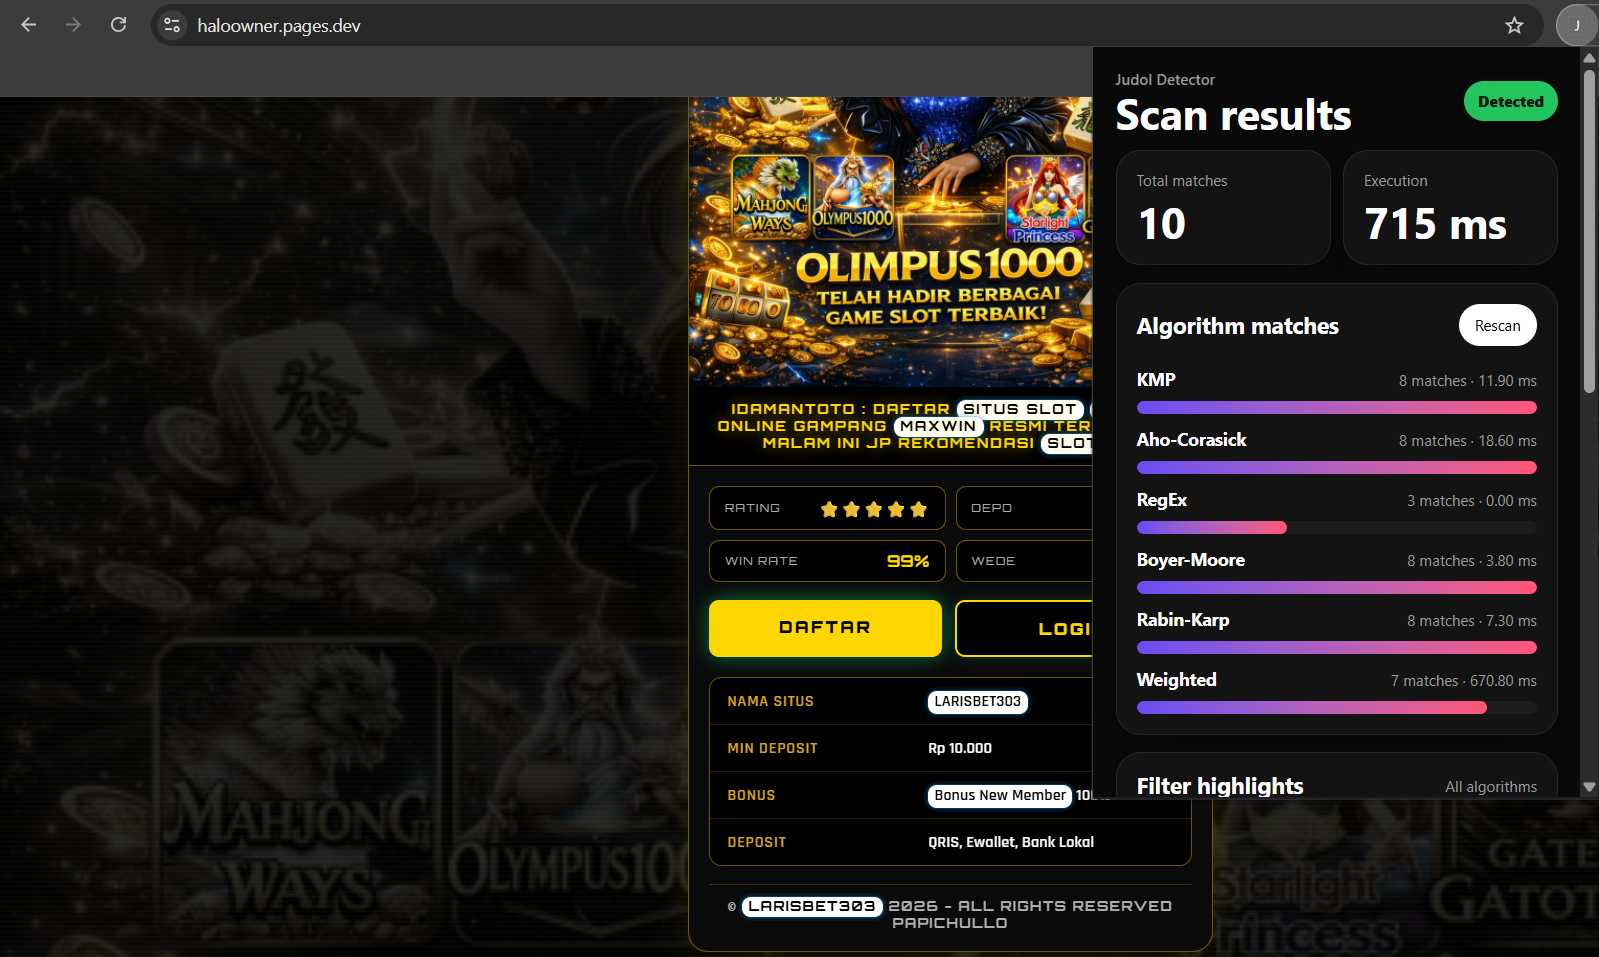
\includegraphics[width=0.92\textwidth]{pengujian/TC1_all.png}
	\caption{TC-01: Hasil pemindaian dengan semua algoritma aktif.}
	\label{fig:tc1-all}
\end{figure}

\begin{figure}[H]
	\centering
	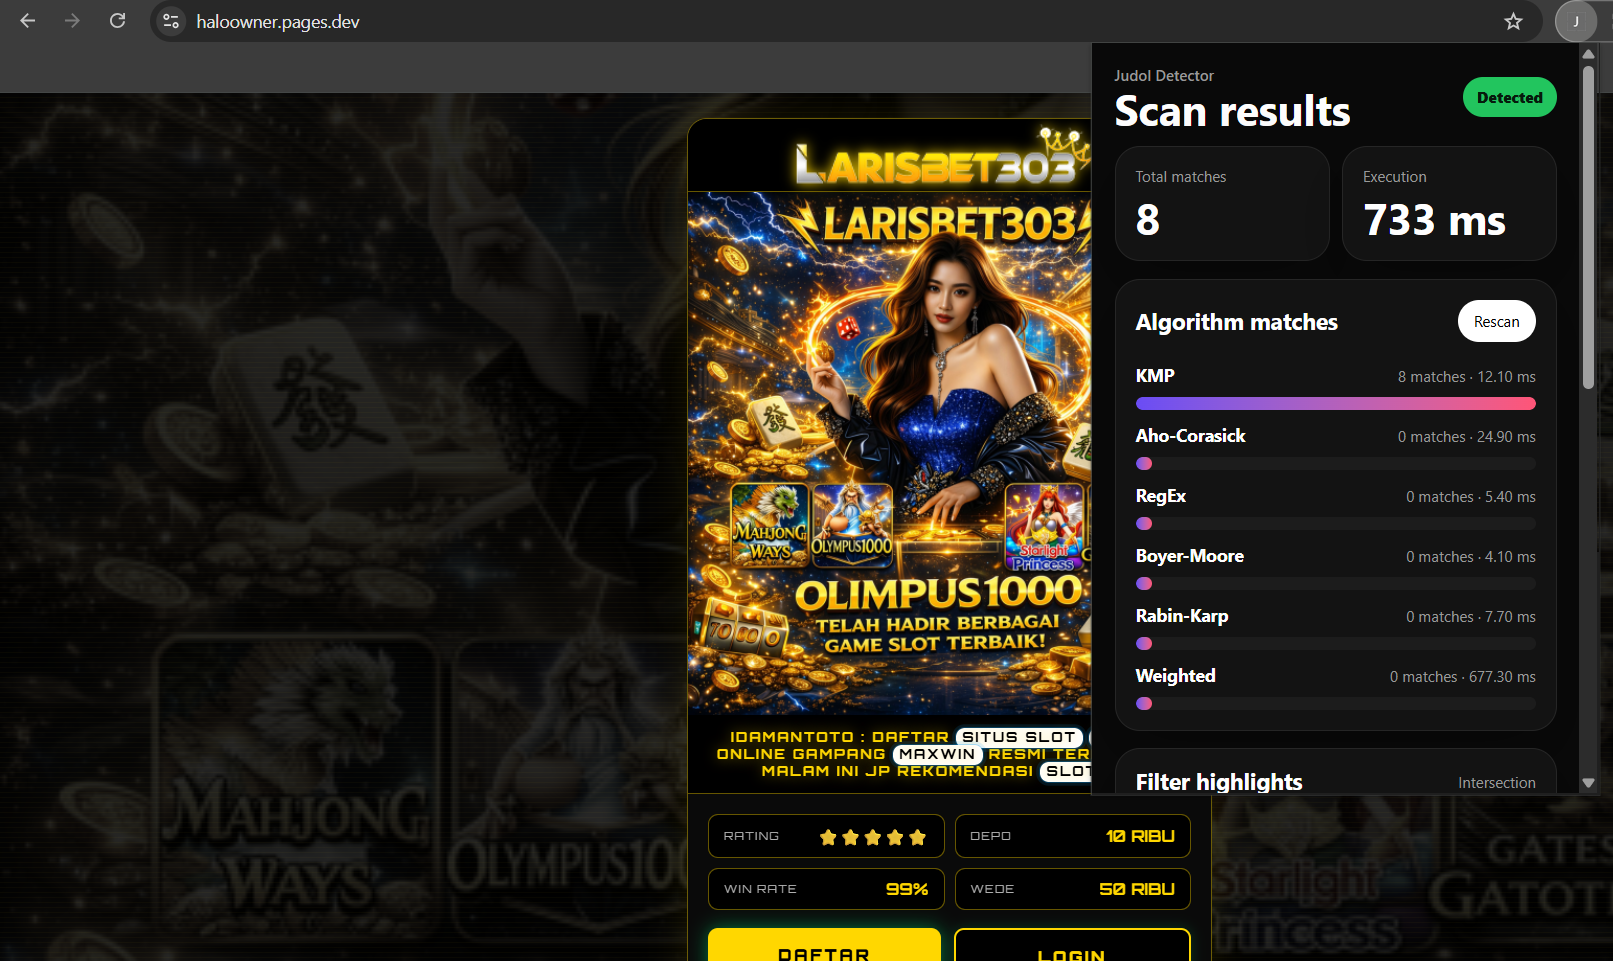
\includegraphics[width=0.92\textwidth]{pengujian/TC1_KMP.png}
	\caption{TC-01: Filter highlight hanya KMP.}
	\label{fig:tc1-kmp}
\end{figure}

\begin{figure}[H]
	\centering
	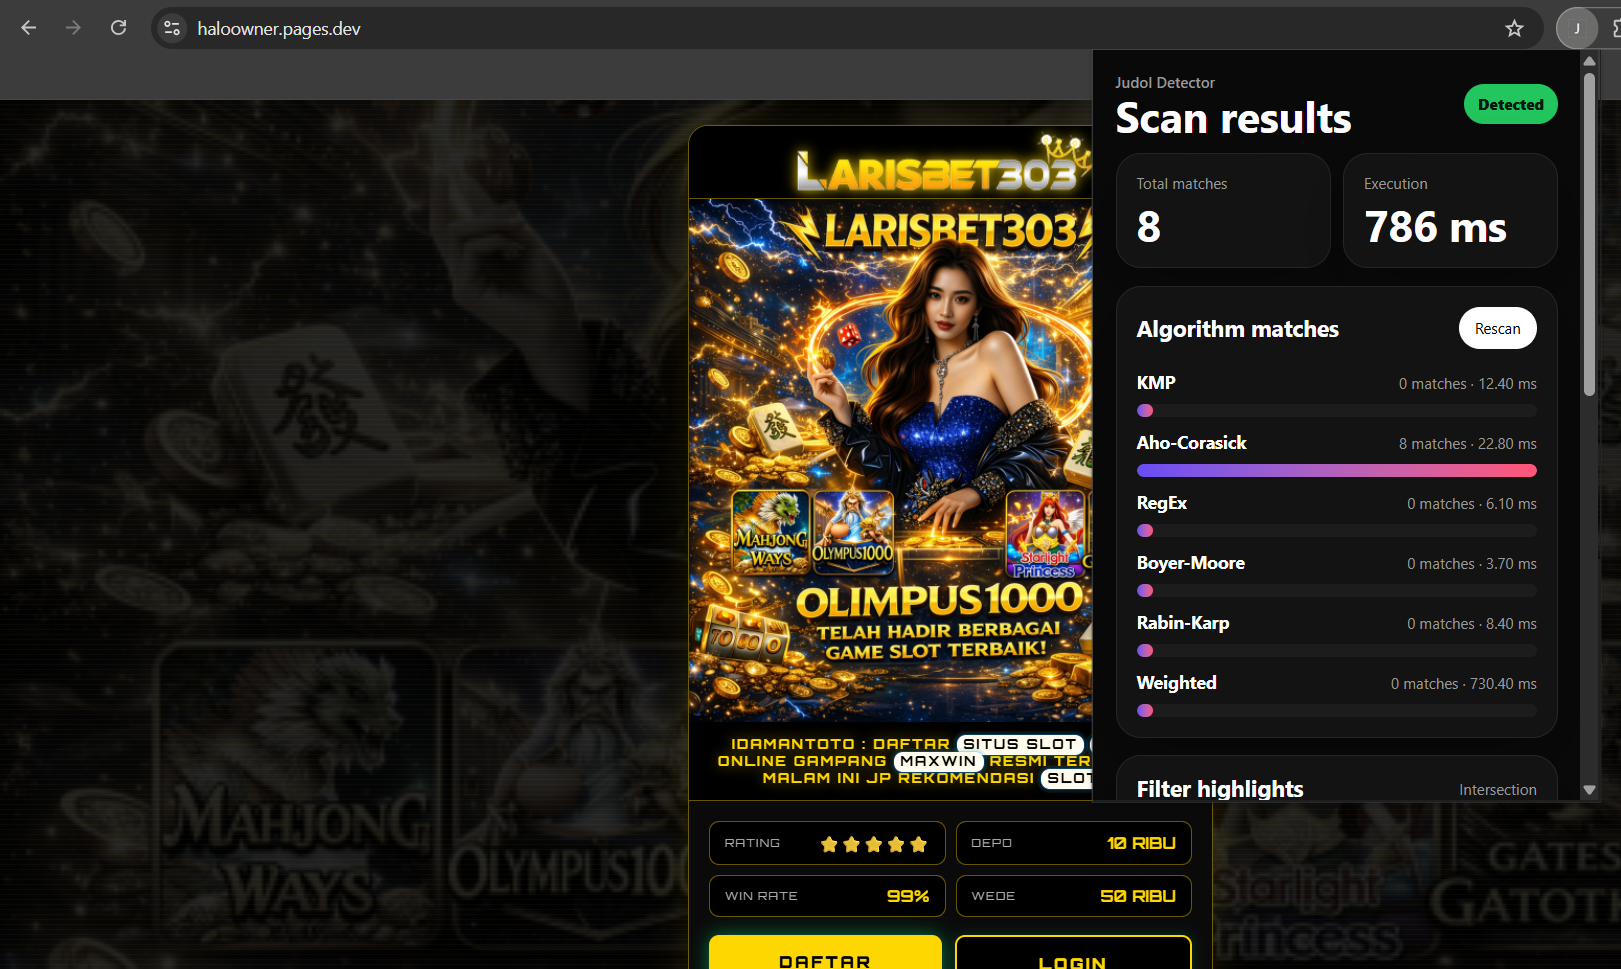
\includegraphics[width=0.92\textwidth]{pengujian/TC1_AC.png}
	\caption{TC-01: Filter highlight hanya Aho-Corasick.}
	\label{fig:tc1-ac}
\end{figure}

\begin{figure}[H]
	\centering
	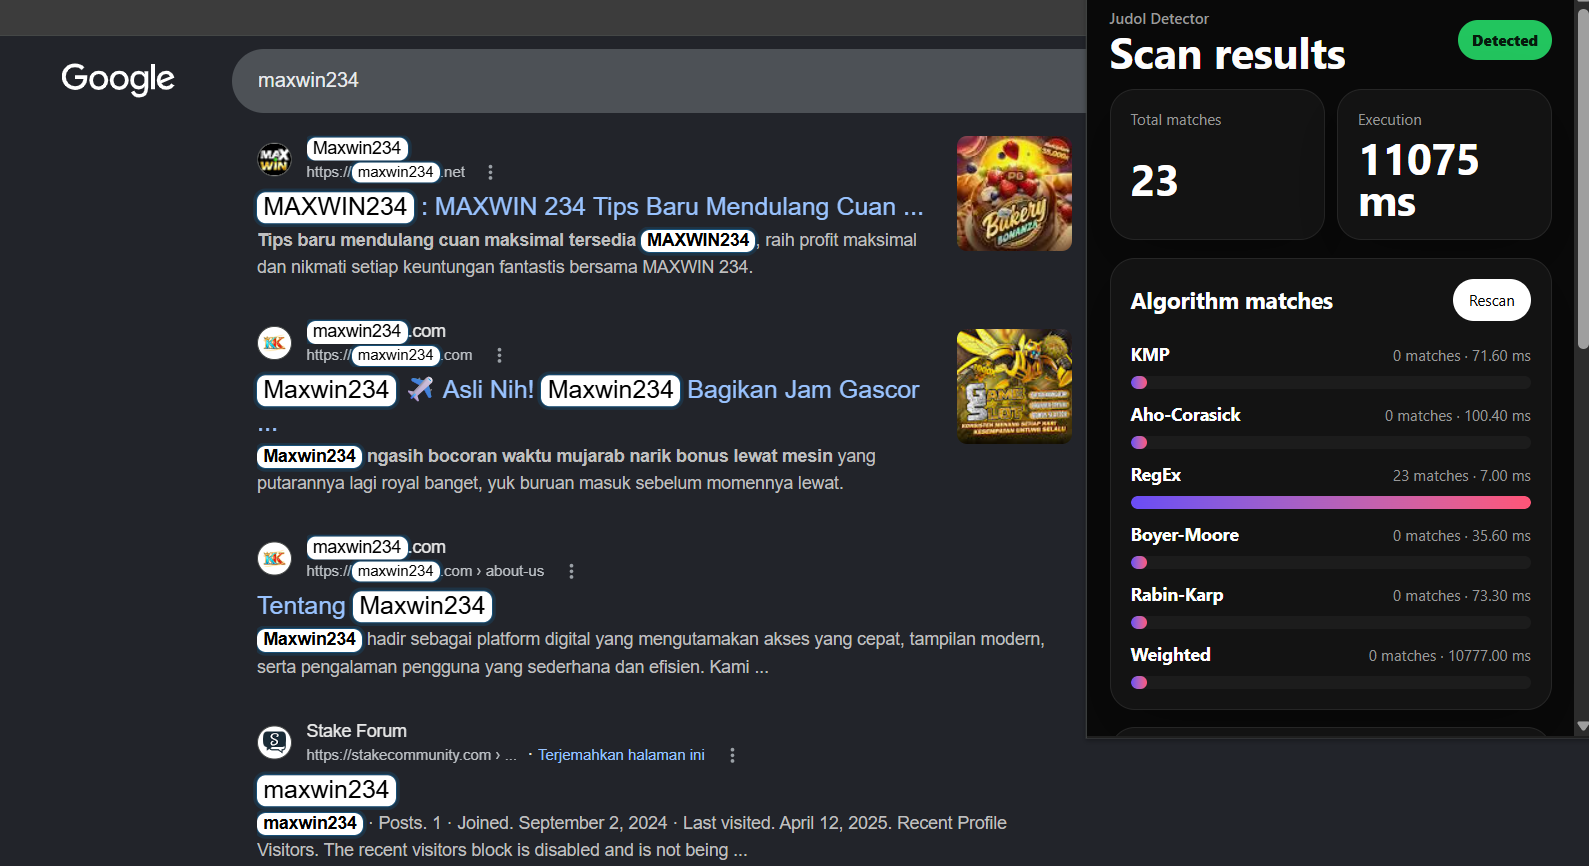
\includegraphics[width=0.92\textwidth]{pengujian/TC2_regex.png}
	\caption{TC-02: Deteksi pola \texttt{MAXWIN234} oleh RegEx.}
	\label{fig:tc2}
\end{figure}

\begin{figure}[H]
	\centering
	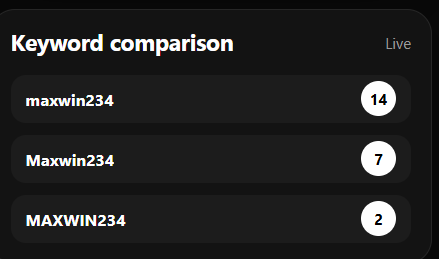
\includegraphics[width=0.92\textwidth]{pengujian/TC2_keyword.png}
	\caption{TC-02: Hasil perbandingan keyword.}
	\label{fig:tc2}
\end{figure}

\begin{figure}[H]
	\centering
	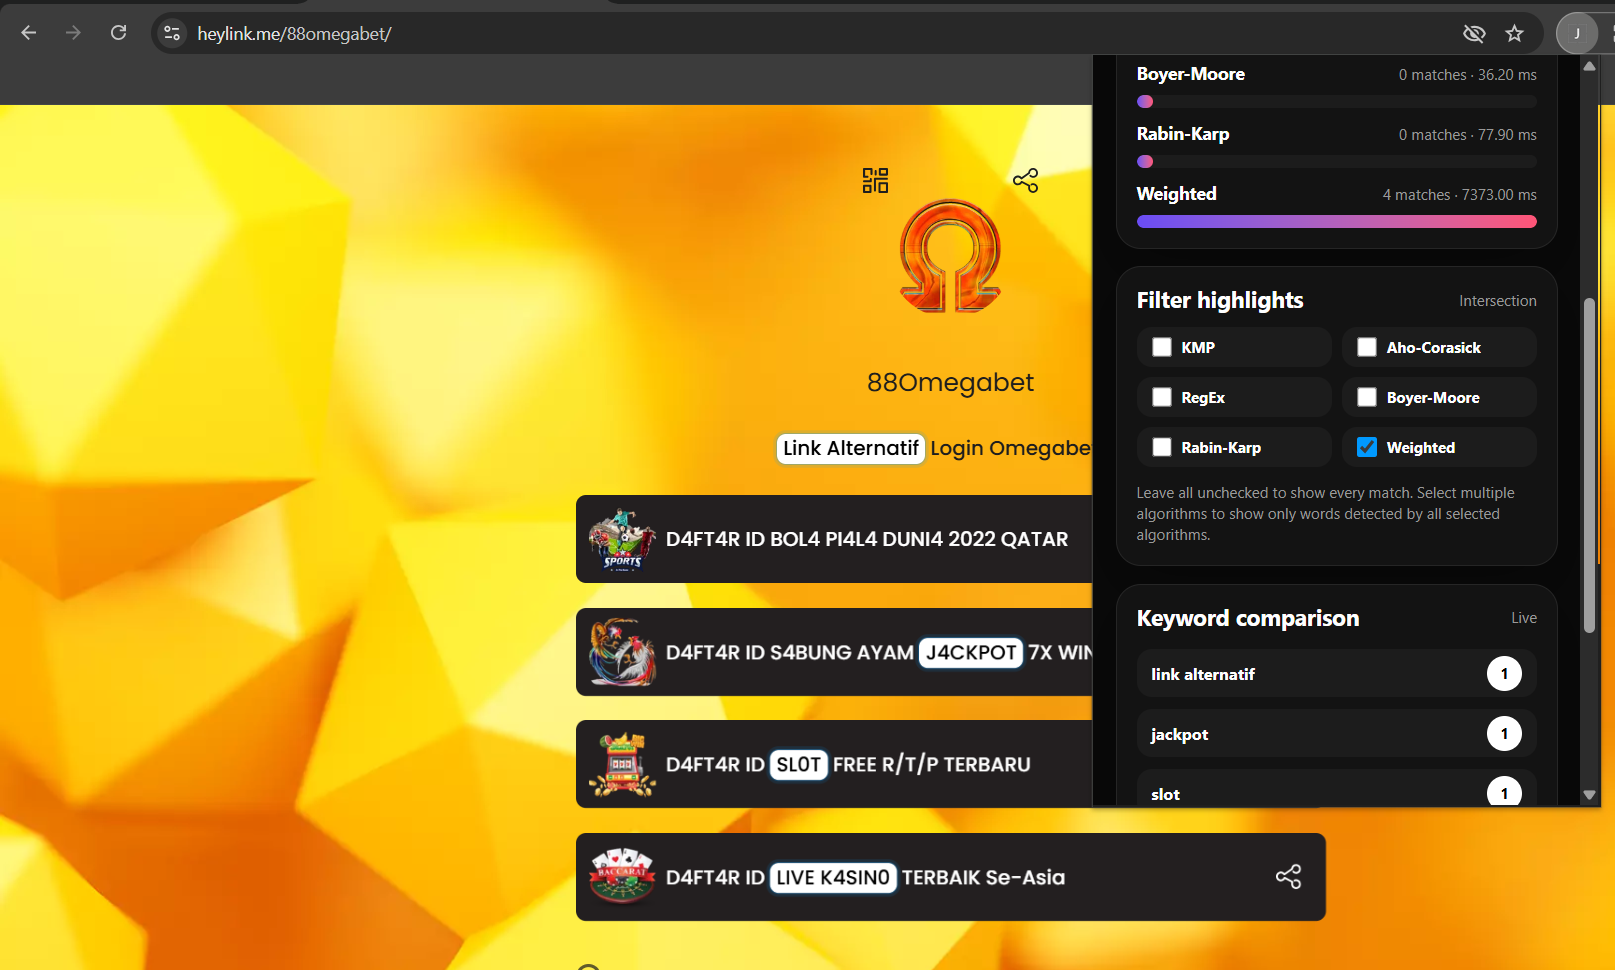
\includegraphics[width=0.92\textwidth]{pengujian/TC3_WL.png}
	\caption{TC-03: Deteksi fuzzy dengan Weighted Levenshtein}
	\label{fig:tc3-wl}
\end{figure}

\begin{figure}[H]
	\centering
	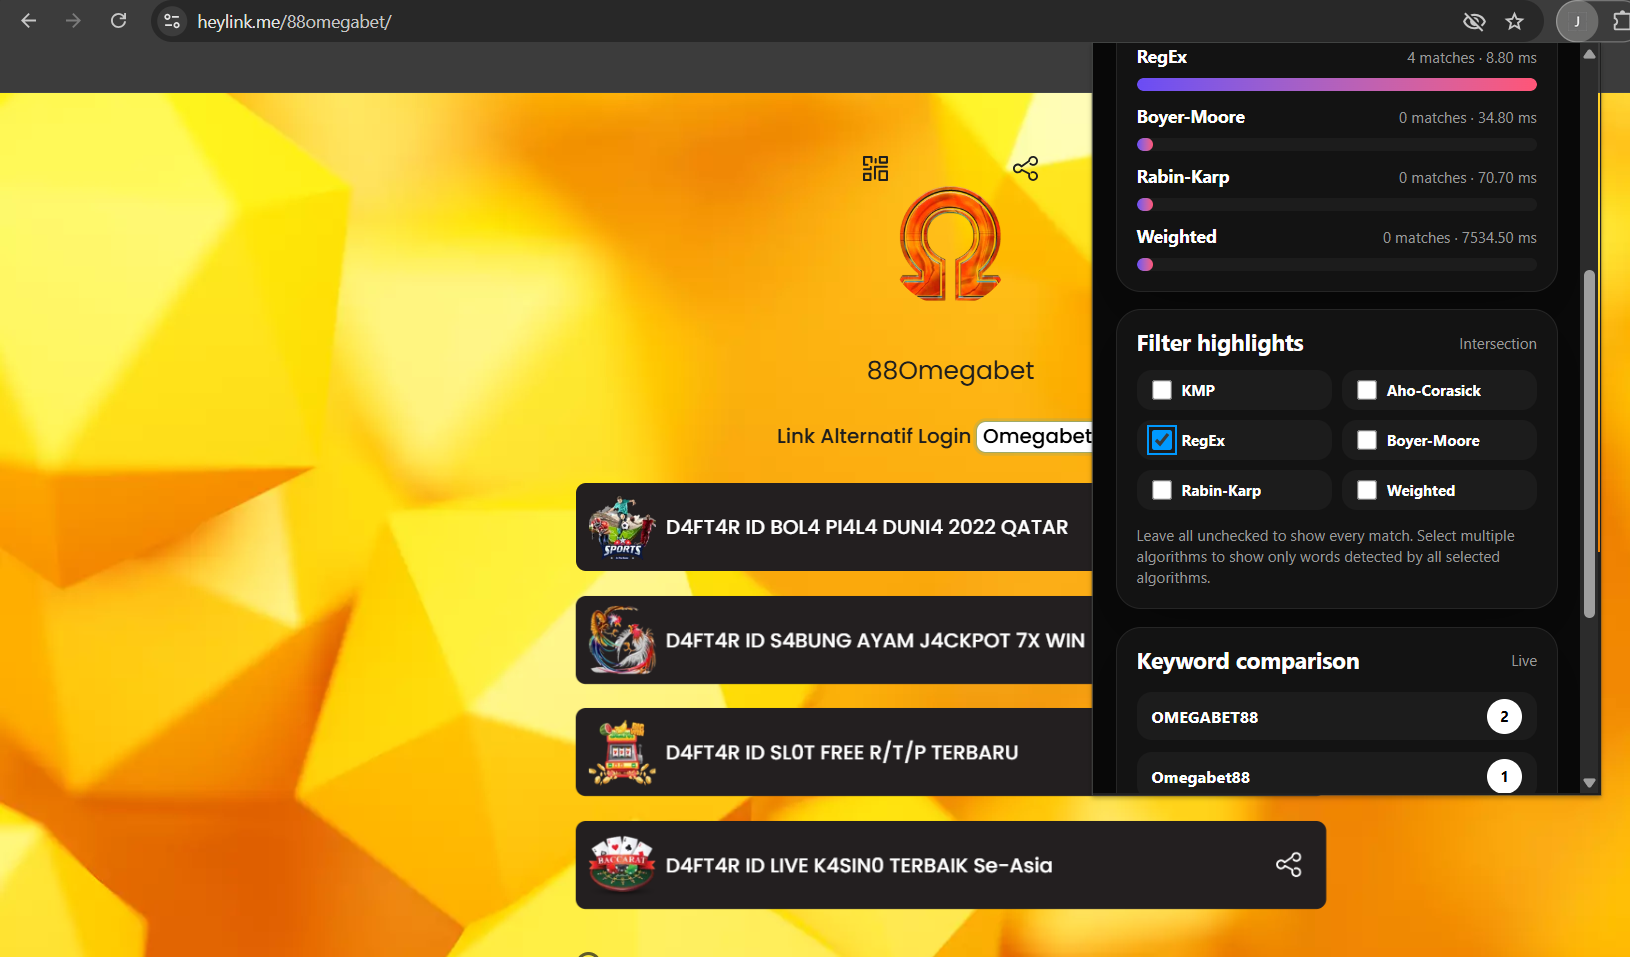
\includegraphics[width=0.92\textwidth]{pengujian/TC3_regex.png}
	\caption{TC-03: Deteksi dengan RegEx}
	\label{fig:tc3-wl}
\end{figure}

\begin{figure}[H]
	\centering
	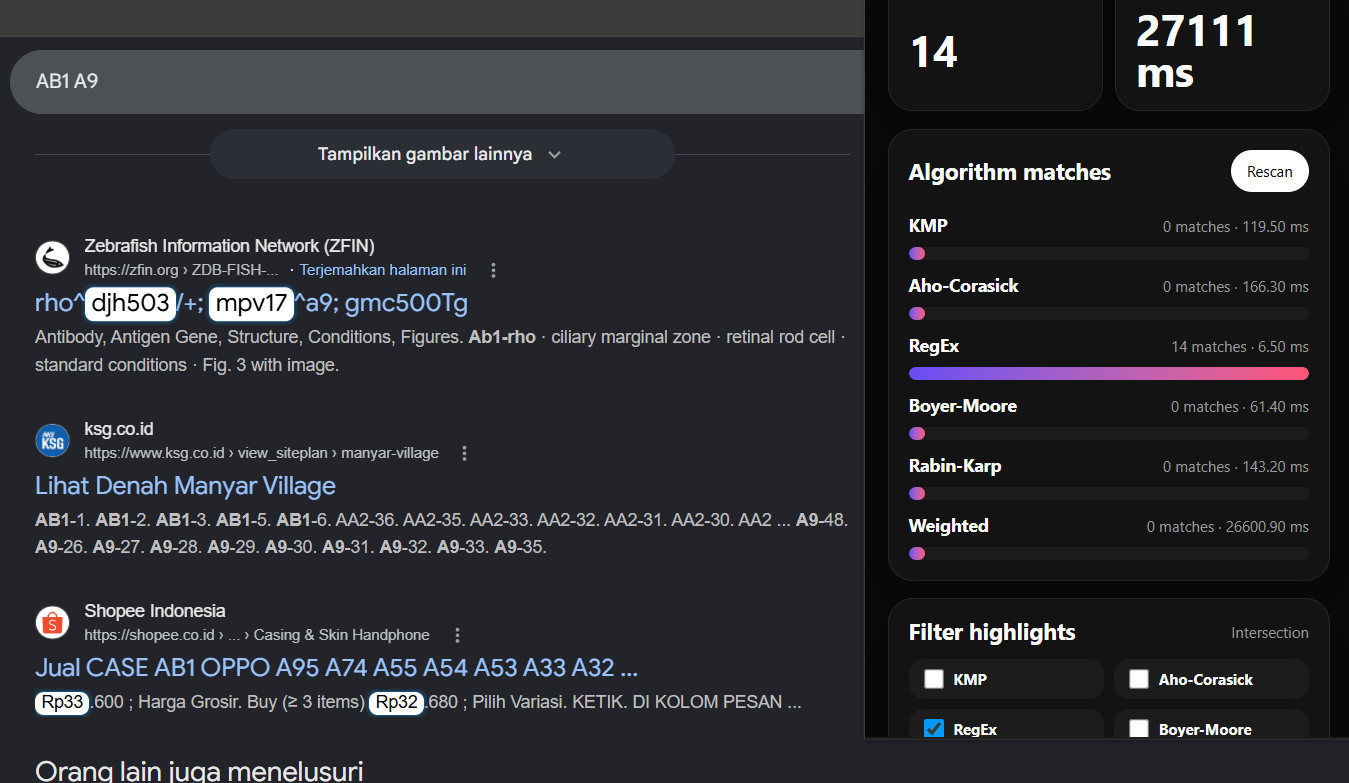
\includegraphics[width=0.92\textwidth]{pengujian/TC4.png}
	\caption{TC-04: Contoh false positive pola RegEx pada token umum.}
	\label{fig:tc4}
\end{figure}

\begin{figure}[H]
	\centering
	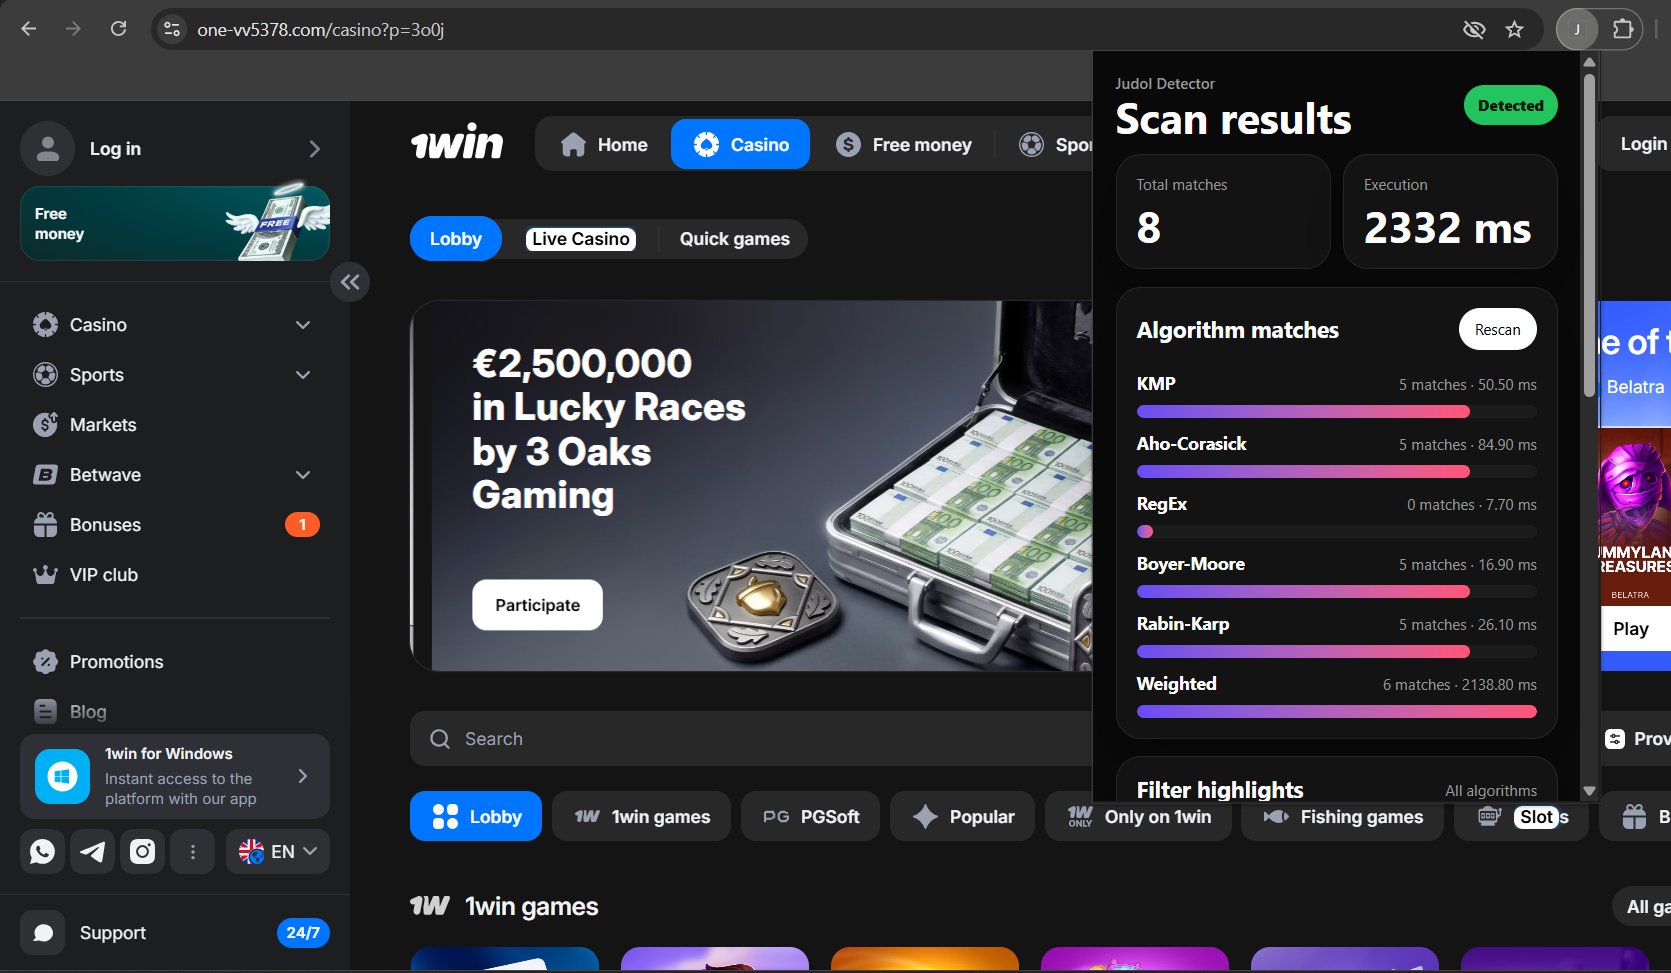
\includegraphics[width=0.92\textwidth]{pengujian/TC5_all.png}
	\caption{TC-05: Deteksi dengan semua algoritma dalam webpage.}
	\label{fig:tc5-all}
\end{figure}

\begin{figure}[H]
	\centering
	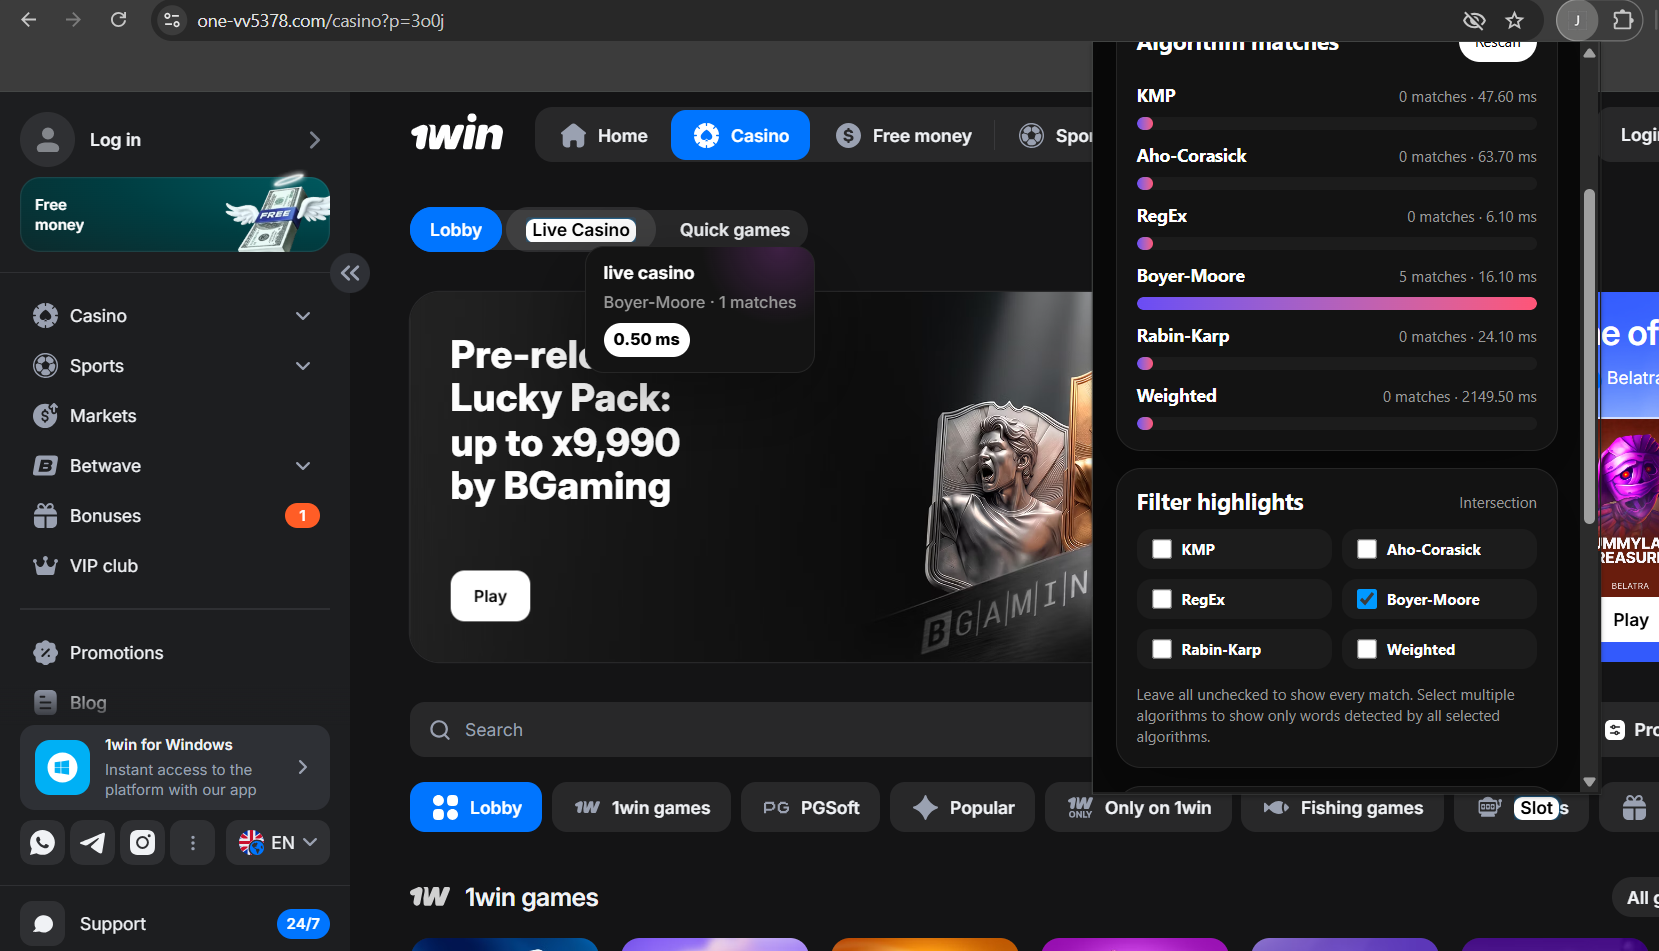
\includegraphics[width=0.92\textwidth]{pengujian/TC5_BM.png}
	\caption{TC-05: Deteksi dengan algoritma Boyer-Moore.}
	\label{fig:tc5-bm}
\end{figure}

\begin{figure}[H]
	\centering
	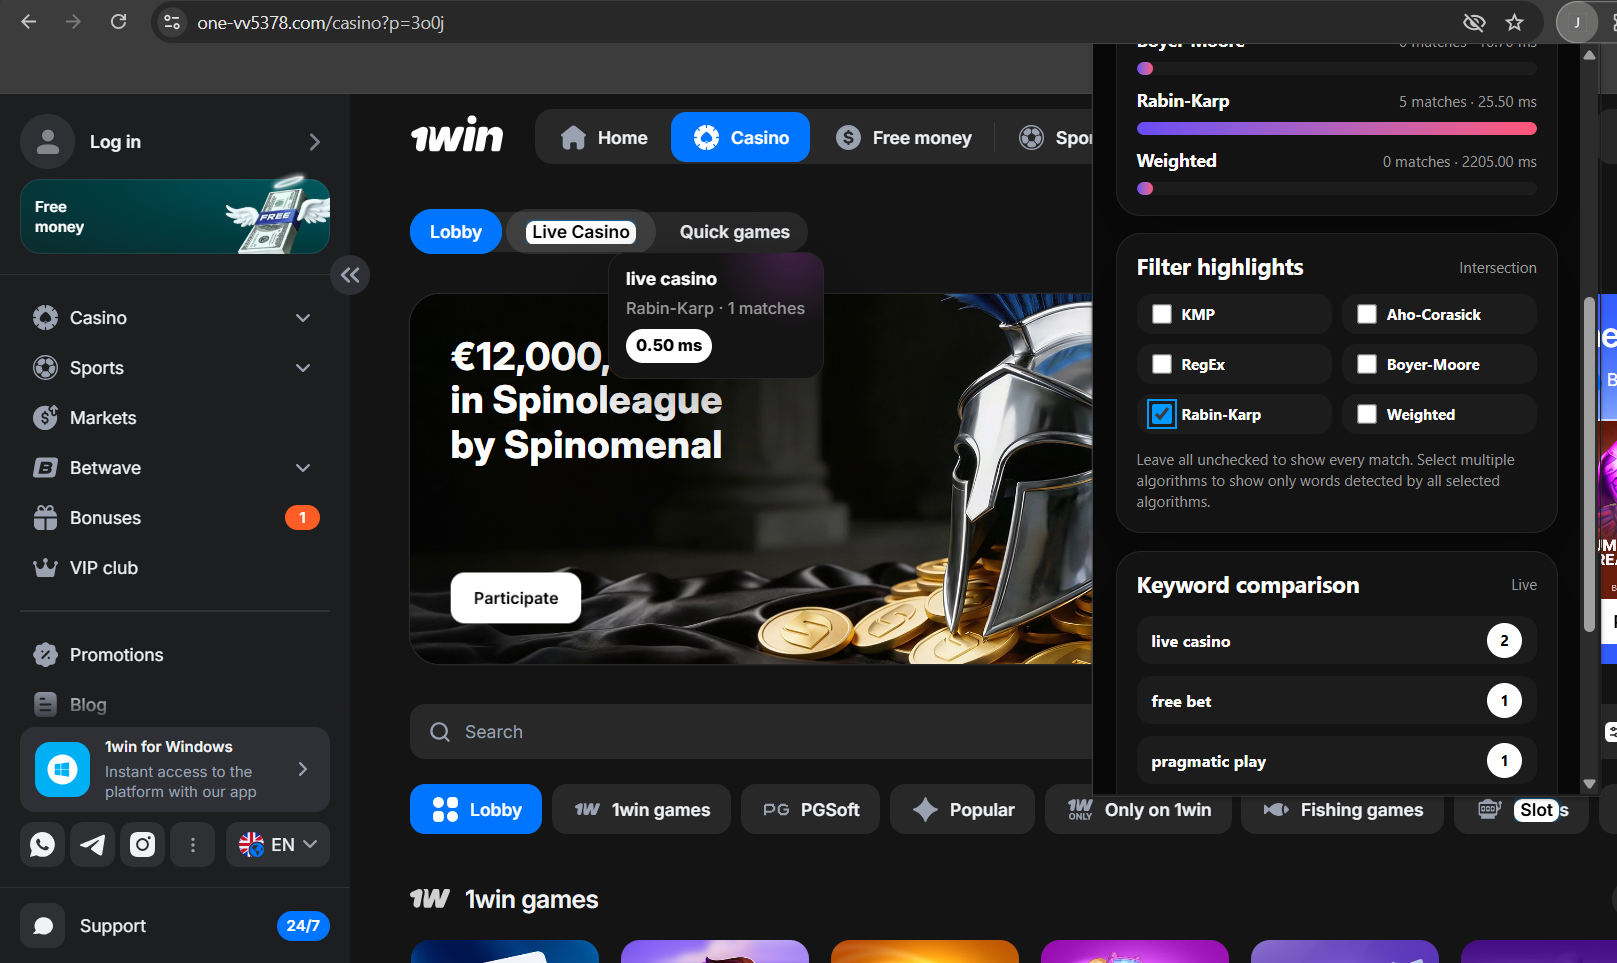
\includegraphics[width=0.92\textwidth]{pengujian/TC5_RK.png}
	\caption{TC-05: Deteksi dengan semua algoritma dalam webpage.}
	\label{fig:tc5-rk}
\end{figure}

\begin{figure}[H]
	\centering
	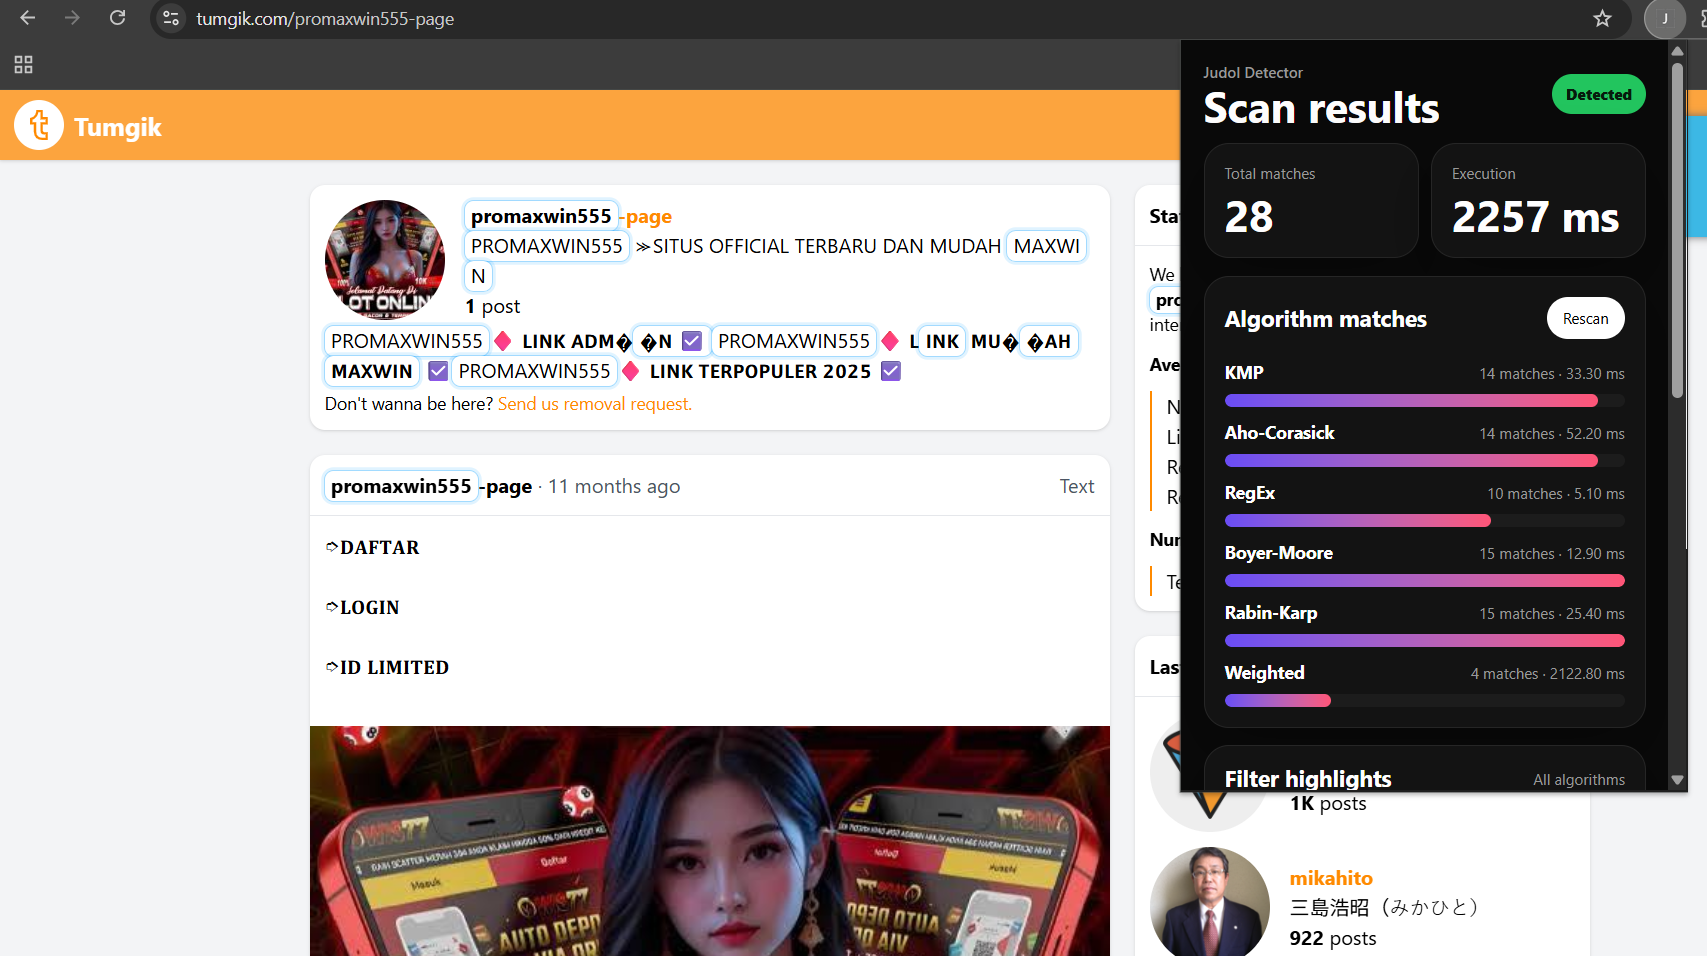
\includegraphics[width=0.92\textwidth]{pengujian/TC6_all.png}
	\caption{TC-06: Deteksi dengan semua algoritma dalam webpage.}
	\label{fig:tc6-all}
\end{figure}

\begin{figure}[H]
	\centering
	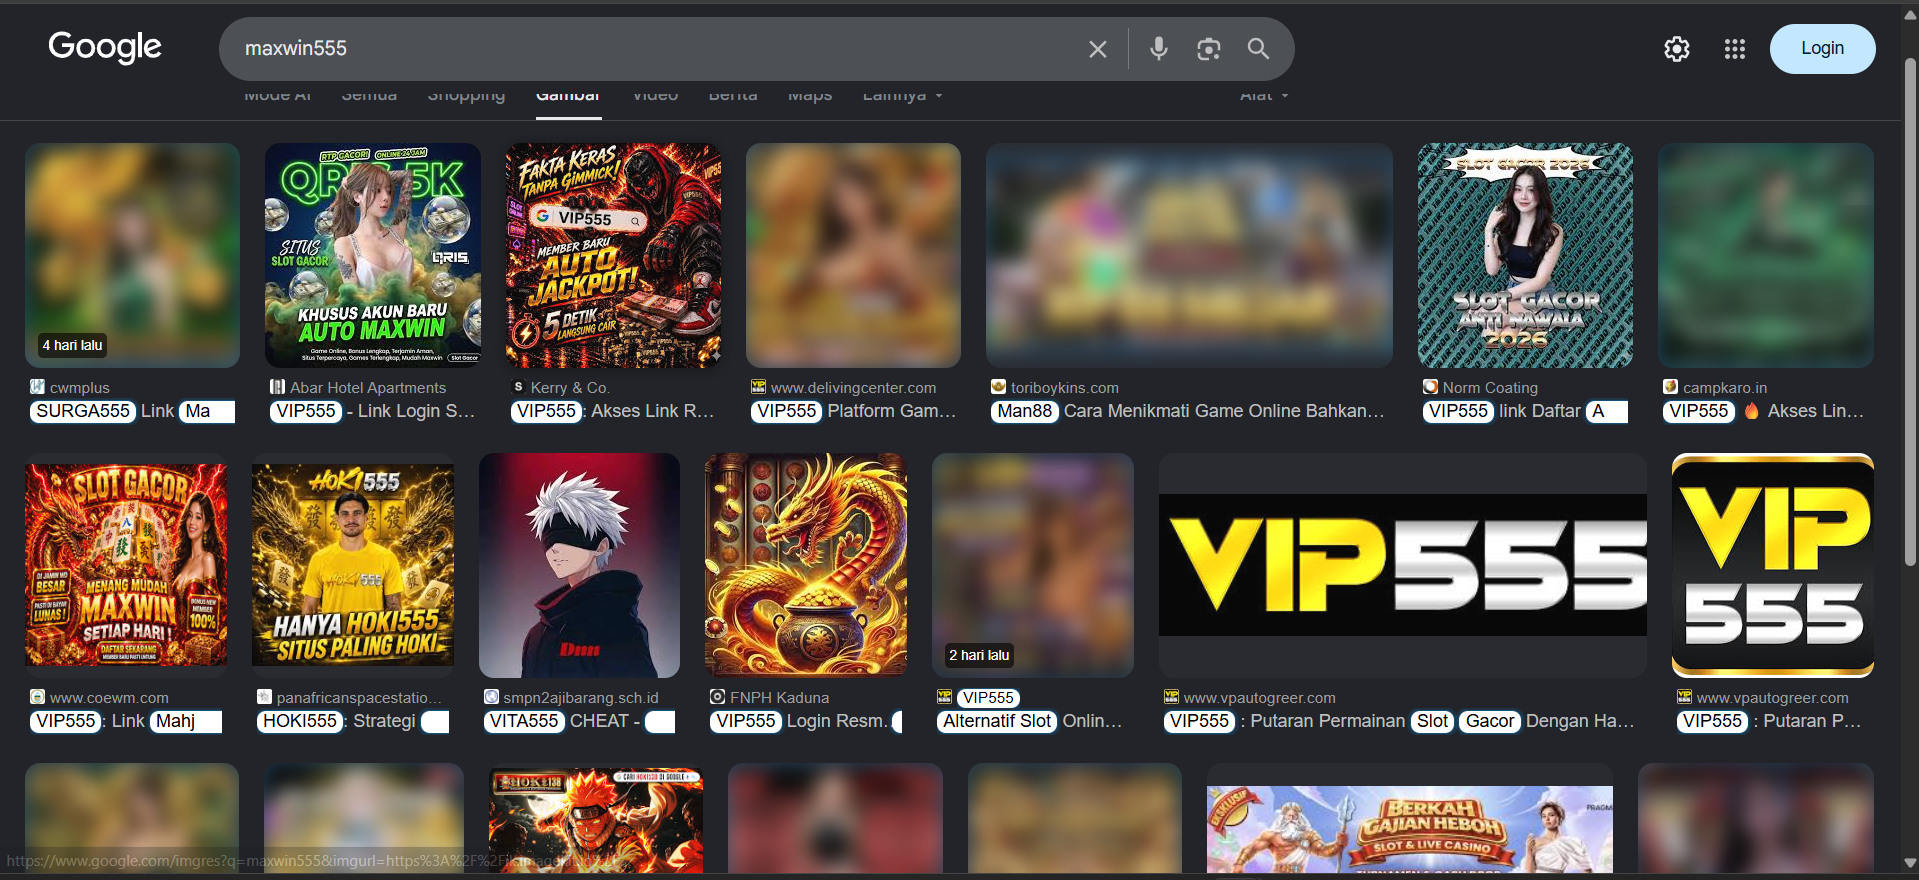
\includegraphics[width=0.92\textwidth]{pengujian/OCR.png}
	\caption{OCR: Deteksi teks pada gambar hasil pencarian gambar.}
	\label{fig:ocr}
\end{figure}

\subsection{Hasil Pengujian}

\begin{table}[H]
\centering
\caption{Hasil pengujian}
\label{tab:hasil-uji}
\begin{tabular}{|p{1.5cm}|p{4.2cm}|p{3.5cm}|p{2.5cm}|}
\hline
\textbf{ID TC} & \textbf{Jenis Algoritma} & \textbf{Banyak Match} & \textbf{Waktu (ms)} \\
\hline
TC-01 & KMP & 8 & 12.10 \\
\hline
TC-01 & Aho-Corasick & 8 & 22.8 \\
\hline
TC-02 & RegEx & 23 & 7.0 \\
\hline
TC-03 & RegEx & 4 & 8.8 \\
\hline
TC-03 & Weighted Levenshtein & 4 & 7373.0 \\
\hline
TC-04 & RegEx & 14 & 6.5 \\
\hline
TC-05 & Boyer-Moore & 5 & 16.1 \\
\hline
TC-05 & Rabin-Karp & 5 & 23.5 \\
\hline
TC-06 & KMP & 14 & 33.3 \\
\hline
TC-06 & Aho-Corasick & 14 & 52.2 \\
\hline
TC-06 & RegEx & 10 & 5.1 \\
\hline
TC-06 & Boyer-Moore & 15 & 12.9 \\
\hline
TC-06 & Rabin-Karp & 15 & 25.4 \\
\hline
TC-06 & Weighted Levenshtein & 4 & 2122.8 \\
\hline
\end{tabular}
\end{table}

\section{Analisis Hasil Pengujian}

Bagian ini membahas perbandingan performa dan akurasi antar algoritma.

\subsection{Perbandingan Performa}

\begin{itemize}
	\item RegEx konsisten menjadi yang tercepat pada semua kasus uji
	(5.1--8.8 ms), karena hanya melakukan pencocokan pola tunggal pada teks.
	Keunggulan: sangat cepat untuk pola sederhana. Kelemahan: mudah memicu
	false positive tanpa konteks.
	\item Algoritma exact matching (KMP, Boyer-Moore, Aho-Corasick, Rabin-Karp)
	berada pada rentang puluhan milidetik; KMP cenderung lebih cepat daripada
	Aho-Corasick pada kasus dengan keyword terbatas (TC-01), sedangkan
	Aho-Corasick tetap stabil ketika jumlah keyword bertambah (TC-06).
	Keunggulan KMP: stabil dan sederhana untuk satu pola. Kelemahan: perlu
	memindai per keyword. Keunggulan Boyer-Moore: lompatan besar saat mismatch,
	baik untuk pola pendek. Kelemahan: performa bisa turun pada teks repetitif.
	Keunggulan Aho-Corasick: satu lintasan untuk banyak keyword. Kelemahan:
	overhead trie dan failure links. Keunggulan Rabin-Karp: hash cepat untuk
	window. Kelemahan: tetap perlu verifikasi saat hash cocok.
	\item Weighted Levenshtein memiliki waktu paling besar (2.1--7.3 detik)
	karena menghitung jarak berbobot pada banyak kandidat token; hal ini
	menunjukkan kebutuhan pembatasan kandidat agar tetap responsif.
	Keunggulan: menangkap variasi visual yang tidak terdeteksi eksak.
	Kelemahan: biaya komputasi tinggi pada teks panjang.
\end{itemize}

\subsection{Pembahasan Akurasi dan False Positive}

\begin{itemize}
	\item Pencocokan eksak (KMP, Boyer-Moore, Aho-Corasick, Rabin-Karp)
	menunjukkan hasil konsisten pada keyword yang benar, terutama pada TC-01
	(8 match) dan TC-06 (14--15 match).
	\item RegEx efektif menangkap pola \texttt{<kata><angka>} pada TC-02 dan
	TC-03, namun menghasilkan false positive pada TC-04 (contoh token umum
	\texttt{AB1}, \texttt{A9}, \texttt{Rp33}, \texttt{Rp32}). Hal ini wajar
	karena pola RegEx belum mempertimbangkan konteks semantik.
	\item Weighted Levenshtein berhasil menemukan variasi visual (TC-03),
	namun biaya komputasinya tinggi. Threshold default 0.78 cukup sensitif
	untuk variasi karakter, tetapi perlu dikontrol agar tidak memicu terlalu
	banyak kandidat pada halaman besar.
	\item OCR memperluas cakupan deteksi ke konten gambar (lihat Gambar
	\ref{fig:ocr}). Hasil OCR efektif untuk menangkap teks judol yang tidak
	tersedia sebagai DOM, namun akurasinya bergantung pada kualitas gambar
	dan bisa menghasilkan teks parsial; karena itu tetap diperlukan validasi
	lewat pipeline string matching untuk mengurangi false positive.
\end{itemize}

\subsection{Ringkasan Analisis}

Secara keseluruhan, pipeline mampu mendeteksi keyword dan pola judol pada
beragam halaman, dengan RegEx dan algoritma exact matching sebagai komponen
tercepat dan paling stabil. Weighted Levenshtein terbukti penting untuk
variasi visual, tetapi perlu digunakan selektif agar performa tetap baik.
Untuk mengurangi false positive, pola RegEx sebaiknya ditambah filter
berdasarkan prefix umum atau konteks kata kunci sekitar.
Keunggulan utama RegEx adalah kecepatan, sementara kelemahannya ada pada
akurasi konteks. KMP dan Boyer-Moore unggul untuk pencocokan eksak dengan
overhead rendah, namun skalanya terbatas saat keyword banyak. Aho-Corasick
memberi keuntungan ketika keyword banyak, tetapi membutuhkan preprocessing
lebih berat. Rabin-Karp efektif untuk pemeriksaan berbasis hash, tetapi
masih memerlukan verifikasi agar aman dari collision. Weighted Levenshtein
memberi fleksibilitas terhadap variasi visual, tetapi menjadi bottleneck
performa tanpa pembatasan kandidat.

	
	\chapter{Penutup}
	\section{Penutup}

Bab ini berisi ringkasan hasil yang diperoleh serta saran untuk pengembangan
lebih lanjut.

\subsection{Kesimpulan}

\begin{enumerate}
	\item \textbf{Judol Detector berhasil menerapkan algoritma pencocokan string}
	(KMP, Boyer-Moore, Aho-Corasick, Rabin-Karp, RegEx, dan Weighted Levenshtein)
	untuk mendeteksi indikasi konten judol pada halaman web.
	\item \textbf{Algoritma RegEx dan exact matching memberikan performa terbaik}
	untuk halaman umum, sedangkan Weighted Levenshtein efektif menangkap
	variasi visual namun memiliki biaya komputasi tinggi.
	\item \textbf{Hasil pengujian menunjukkan kebutuhan pengendalian false positive,}
	terutama pada pola RegEx yang dapat menangkap token umum tanpa konteks.
\end{enumerate}

\subsection{Saran}

\begin{enumerate}
	\item \textbf{Tambahkan filter konteks untuk RegEx} misalnya pengecualian
	prefix umum atau verifikasi dengan keyword sekitar agar false positive
	berkurang.
	\item \textbf{Optimasi Weighted Levenshtein dengan pembatasan kandidat} dan
	pengaturan threshold adaptif agar performa tetap responsif pada halaman besar.
\end{enumerate}


	\chapter{Lampiran}
	\section{Lampiran}

\subsection{Pernyataan Tidak Melakukan Kecurangan}
\noindent
\fbox{
  \begin{minipage}{\dimexpr\linewidth-2\fboxsep-2\fboxrule\relax}
    \vspace{0.2cm}
    Tugas ini disusun sepenuhnya tanpa bantuan kecerdasan buatan (\textit{Generative AI}), melainkan hasil pemikiran dan analisis mandiri.
    
    \begin{flushright}
      \vspace{0.5cm}
      
\includegraphics[width=3cm]{public/nus.jpeg} \\
      {Stevanus Agustaf Wongso} \\[0.5cm]
      
      
\includegraphics[width=3cm]{public/wen.png} \\
      {Ray Owen Martin} \\[0.5cm]
      
      
\includegraphics[width=3cm]{public/atil.jpeg} \\
      {Athilla Zaidan Zidna Fann} \\[0.5cm]
      \vspace{0.2cm}
    \end{flushright}
  \end{minipage}
}

\subsection{Tautan Repository Github}

Repository Github untuk proyek ini dapat diakses di: \url{https://github.com/AthillaZaidan/Tubes3_Pasti-Gacor-Zeus}

\subsection{Tabel Checklist Spesifikasi}
\begin{table}[H]
    \centering
    \renewcommand{\arraystretch}{1.5} 
    \begin{tabular}{|c|p{10cm}|c|c|}
        \hline
        \textbf{No} & \multicolumn{1}{c|}{\textbf{Poin}} & \textbf{Ya} & \textbf{Tidak} \\
        \hline
        1 & Extension berhasil di-build dan di-load tanpa kesalahan pada chromium browser dan dikembangkan dengan TypeScript & v & \\
        \hline
        2 & KMP dan Boyer-Moore diimplementasikan \textit{from scratch} & v & \\
        \hline
        3 & Regex menghandle format \textless kata\textgreater\textless angka\textgreater\ dan berbagai \textit{edge case} & v & \\
        \hline
        4 & Pencarian KMP \& BM membaca \texttt{keyword.txt} secara iteratif dan tidak menggunakan \textit{built-in search function} atau \textit{library} eksternal & v & \\
        \hline
        5 & \textit{Exact matching} dan \textit{fuzzy matching} berjalan benar & v & \\
        \hline
        6 & Elemen DOM terdeteksi diberi \textit{highlight} dan terhapus saat \textit{rescanning} & v & \\
        \hline
        7 & \textit{Tooltip} muncul saat \textit{hover} dengan informasi \textit{keyword}, algoritma, kemunculan, dan waktu eksekusi & v & \\
        \hline
        8 & \textit{Popup} menampilkan statistik \textit{realtime} (total \textit{keyword}, perbandingan, waktu eksekusi, jumlah \textit{match}) & v & \\
        \hline
        9 & {[Bonus]} Membuat Video & & v \\
        \hline
        10 & {[Bonus]} Implementasi Algoritma Aho-Corasick dan Rabin Karp & v & \\
        \hline
        11 & {[Bonus]} Implementasi \textit{Censorship} / \textit{Blur} Teks & v & \\
        \hline
        12 & {[Bonus]} Implementasi \textit{Optical Character Recognition} pada Gambar & v & \\
        \hline
    \end{tabular}
\end{table}

\subsection{Tabel Pembagian Tugas}
\begin{table}[H]
    \centering
    \renewcommand{\arraystretch}{1.5}
    \begin{tabular}{|p{5cm}|p{8cm}|}
        \hline
        Nama & Bagian \\
        \hline
        Stevanus Agustaf Wongso & Rabin-Karp dan Boyer-Moore, laporan \\
        \hline
        Ray Owen Martin & KMP dan Aho-Corasick, laporan \\
        \hline
        Athilla Zaidan Zidna Fann & RegEx, Weighted Levenshtein, OCR, censorship, laporan \\
        \hline
    \end{tabular}
\end{table}


	
	\bibliography{dafpus}
	
\end{document}
